% Type of the document
\documentclass{beamer}

% elementary packages:
\usepackage{graphicx}
\usepackage[latin1]{inputenc}
\usepackage[T1]{fontenc}
\usepackage[english]{babel}
\usepackage{listings}
\usepackage{xcolor}
\usepackage{eso-pic}
\usepackage{mathrsfs}
\usepackage{url}
\usepackage{amssymb}
\usepackage{amsmath}
\usepackage{animate}
\usepackage{multirow}
\usepackage{hyperref}
\usepackage{booktabs}
%\usepackage[demo]{graphicx}
\usepackage{subfig}
%\usepackage{tabularx}
%\usepackage{pgfplotstable}
% recommended:
%\usepackage{booktabs}
%\usepackage{array}
\usepackage{colortbl}

% additional packages
\usepackage{bbm}

% packages supplied with ise-beamer:
\usepackage{cooltooltips}
\usepackage{colordef}
\usepackage{beamerdefs}
\usepackage{lvblisting}
\definecolor{LightCyan}{rgb}{0.88,1,1}
% Change the pictures here:
% logobig and logosmall are the internal names for the pictures: do not modify them. 
% Pictures must be supplied as JPEG, PNG or, to be preferred, PDF
\pgfdeclareimage[height=4.5cm]{logobig}{LogoIRTG}
% Supply the correct logo for your class and change the file name to "logo". The logo will appear in the lower
% right corner:
\pgfdeclareimage[height=0.7cm]{logosmall}{figures/coauthorship}

% Title page outline:
% use this number to modify the scaling of the headline on title page
\renewcommand{\titlescale}{1.0}
% the title page has two columns, the following two values determine the percentage each one should get
\renewcommand{\titlescale}{1.0}
\renewcommand{\leftcol}{0.6}

% Define the title.Don't forget to insert an abbreviation instead 
% of "title for footer". It will appear in the lower left corner:
\title[Network]{Network Centrality}
% Define the authors:
\authora{Ya Qian}
\authorb{Wolfgang Karl H\"ardle}
\authorc{}

% Define any internet addresses, if you want to display them on the title page:
\def\linka{lvb.wiwi.hu-berlin.de}
\def\linkb{\\case.hu-berlin.de}
\def\linkc{\\irtg1792.hu-berlin.de}
% Define the institute:
\institute{Ladislaus von Bortkiewicz Chair of Statistics\\
C.A.S.E. -- Center for Applied Statistics\\
and Economics\\
Humboldt-Universit\"at zu Berlin\\}

% Comment the following command, if you don't want, that the pdf file starts in full screen mode:
\hypersetup{pdfpagemode=FullScreen}

%Start of the document
\begin{document}

% create the title slide, layout controlled in beamerdefs.sty and the foregoing specifications
\frame[plain]{
\titlepage
}

\section{Motivation}
%\frame{
%\frametitle{Network is Everywhere}
%\begin{figure}
%\begin{center}
%\includegraphics[scale=0.15]{Full-Network-Region-Degree-Fruchterman-Reingold-12K-4000x4000-1024x1024.jpg}%\vspace{-0.5cm}
%\caption{Climate Change Network} %\hspace{2cm}
%\href{http://www.pacificrisa.org/projects/social-network-analysis/full-network/}{\textbf{http://www.pacificrisa.org}}
%\end{center}
%\end{figure}
%}


\frame{
\frametitle{International Trade Network}
\begin{figure}
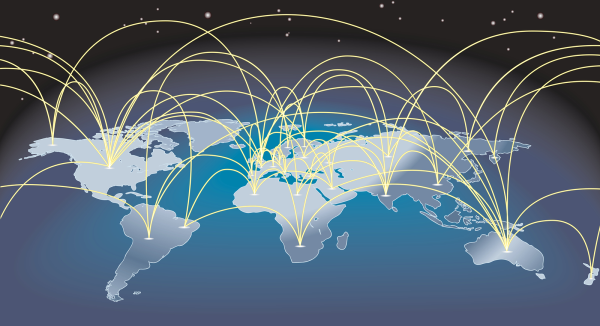
\includegraphics[scale=0.35]{figures/worldtrade}
\caption{International trade picture}
\bigskip
\scriptsize{
\href{http://www.fshcc.com/florida-international-trade-articles/bid/101346/Global-Trade-is-Big-Business-in-Florida}{From Florida State Hispanic Chamber of Commerce}}
\end{figure}
}

\frame{
\frametitle{Production Network}
\begin{figure}
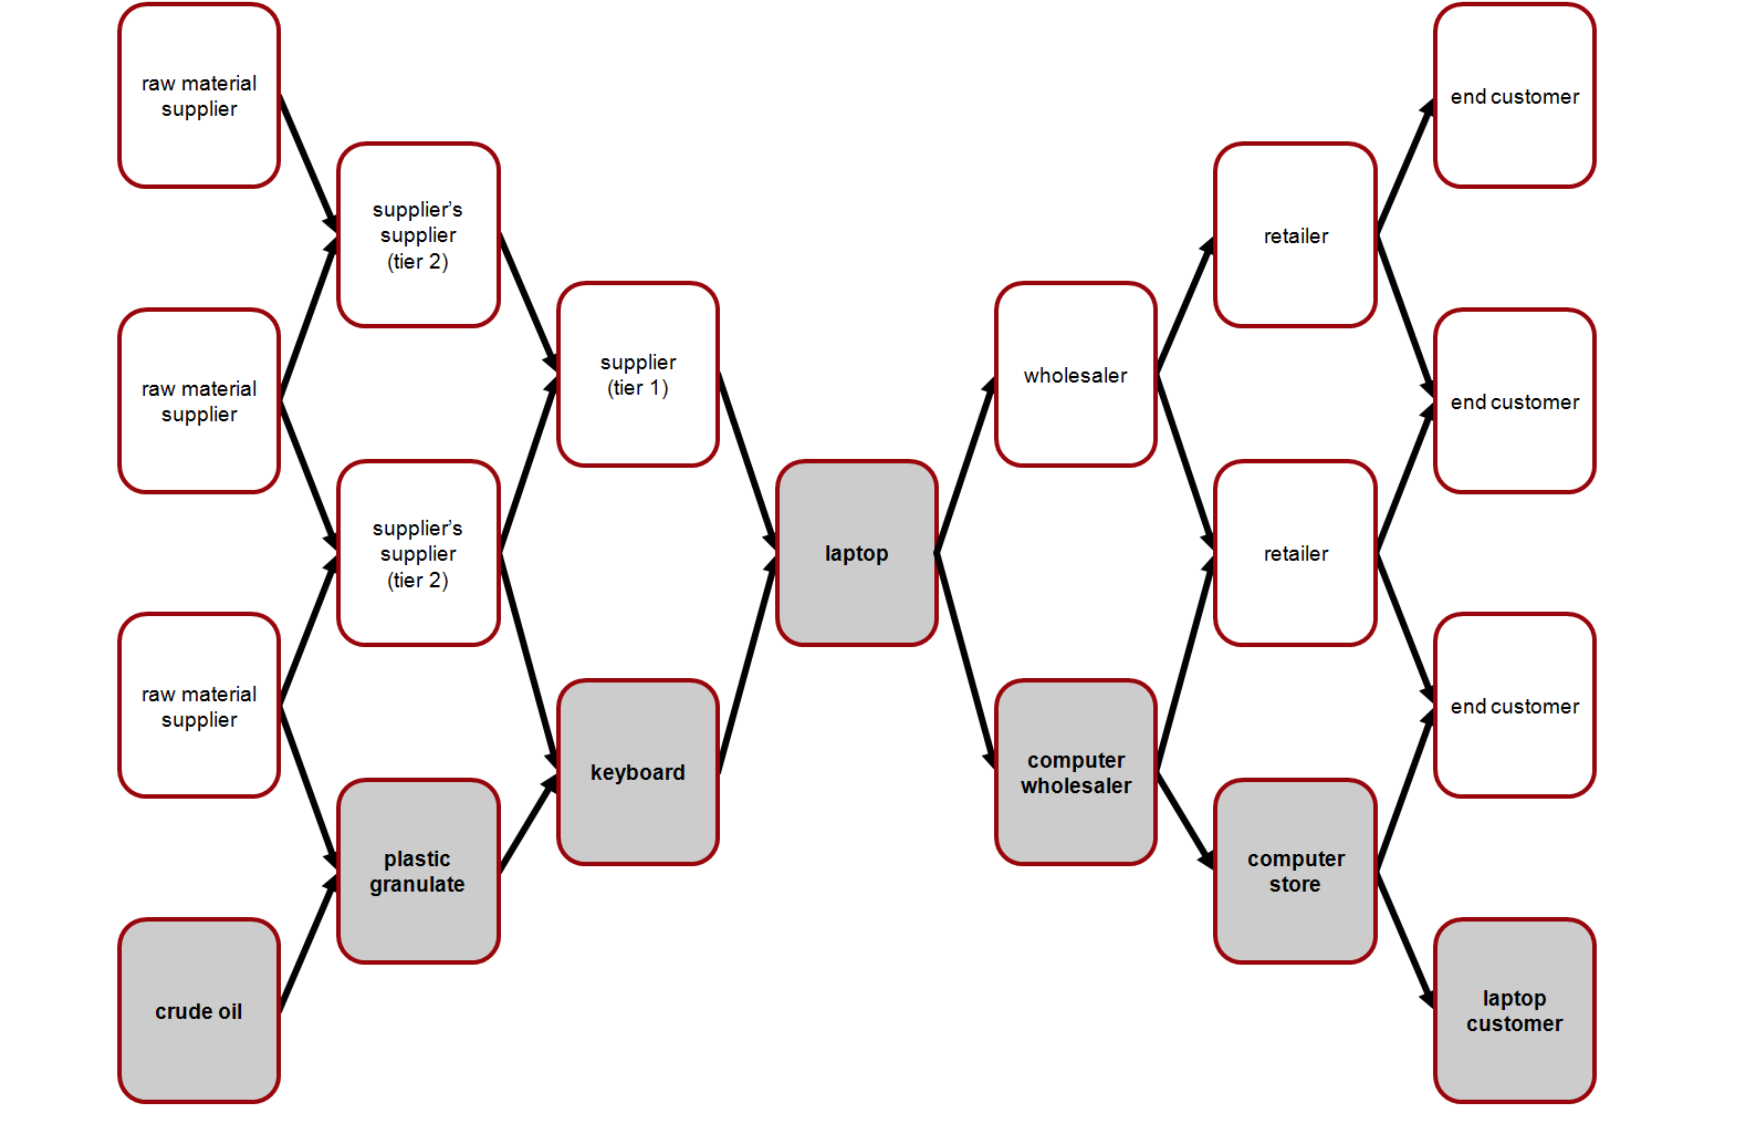
\includegraphics[scale=0.25]{figures/supplychain}
\caption{Supply chain}
\bigskip
\scriptsize{
\href{https://en.wikipedia.org/wiki/Supply_chain}{From Wikipedia}}
\end{figure}
}


\frame{
\frametitle{Social Network}
\begin{figure}
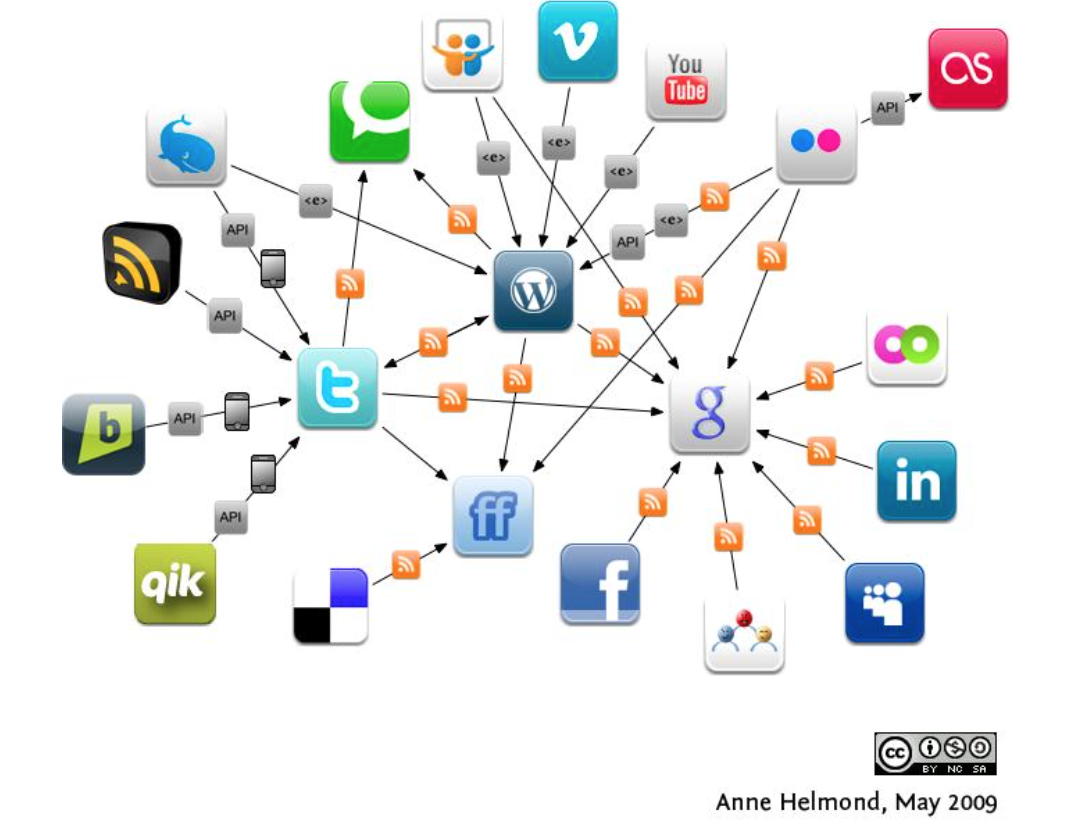
\includegraphics[scale=0.25]{figures/socialnetworks}
\caption{A sample of social network}
\bigskip
\scriptsize{
\href{http://kikolani.com/becoming-accessible-social-networking-social-media.html}{From Webpage Kikolani}}
\end{figure}
}

\frame{
\frametitle{International Financial Network}
\begin{figure}
\includegraphics[scale=0.25]{figures/INFinancialnet}
\caption{A sample of international financial network}
\bigskip
\scriptsize{
From Frank Schweitzer, et al. (Science 325, 422 (2009))}
\end{figure}
}

\frame{
\frametitle{Network of Coauthorship}
\begin{figure}
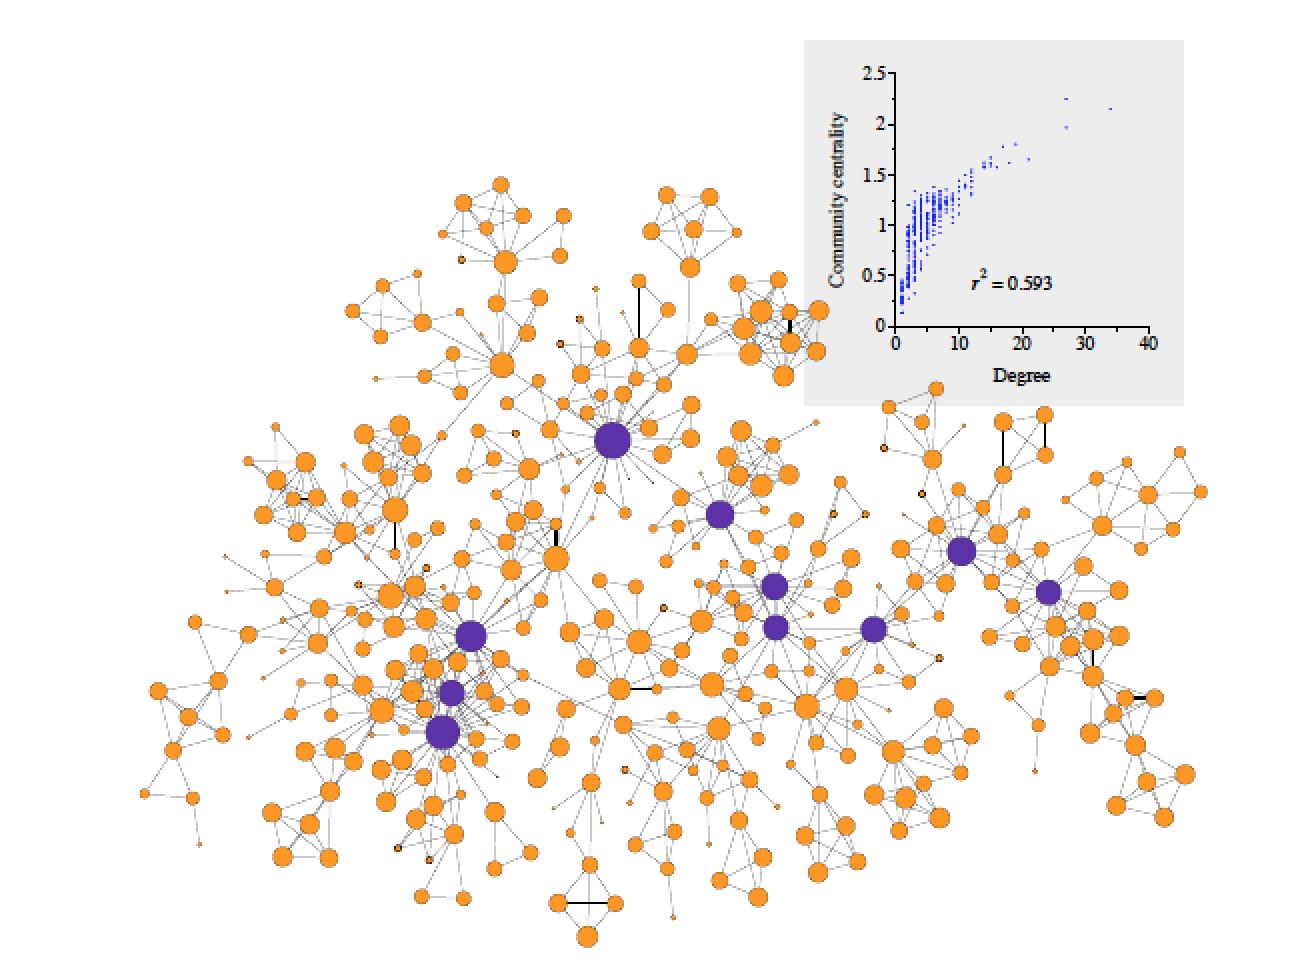
\includegraphics[scale=0.25]{figures/coauthorship}
\caption{A network of coauthorships between 379 scientists whose research centers on the properties of networks of one kind or another}
\bigskip
\scriptsize{
From M.E.J. Newman (Phys. Rev. E 74, 036104 (2006))}
\end{figure}
}

\frame{
\frametitle{A More Specific Coauthorship Graph}
\begin{figure}
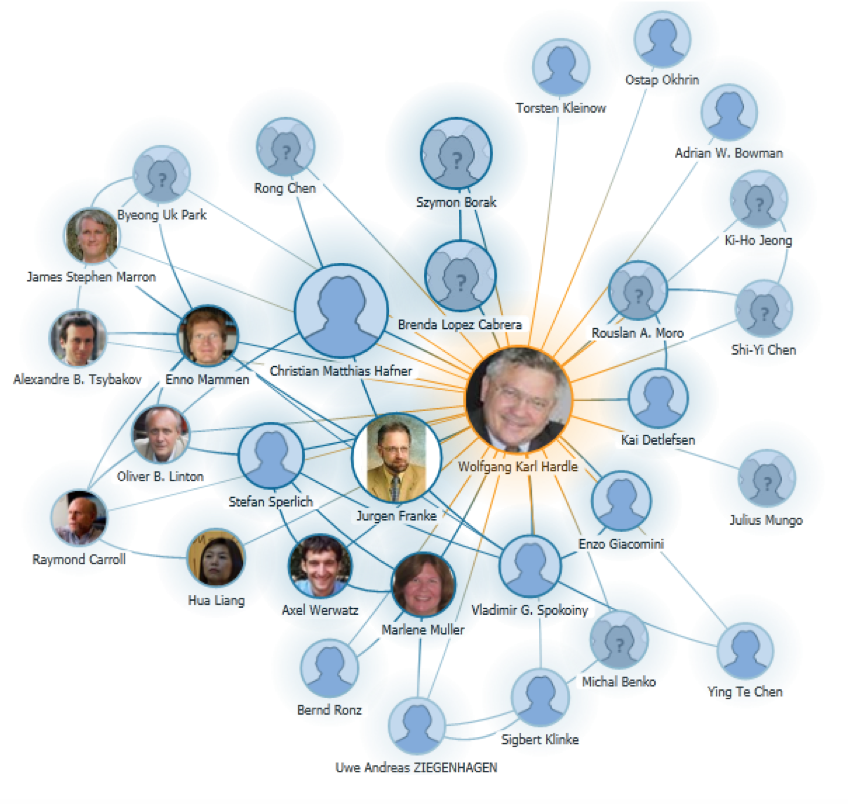
\includegraphics[scale=0.34]{figures/coauthorgraph.png}
\caption{Coauthorship graph of W.K. H\"ardle}
\bigskip
\scriptsize{
\href{http://academic.research.microsoft.com/VisualExplorer\#12530409}
{Source: Microsoft Academic}}
\end{figure}
}

\frame{
\frametitle{A More Specific Coauthorship Graph}
\begin{figure}
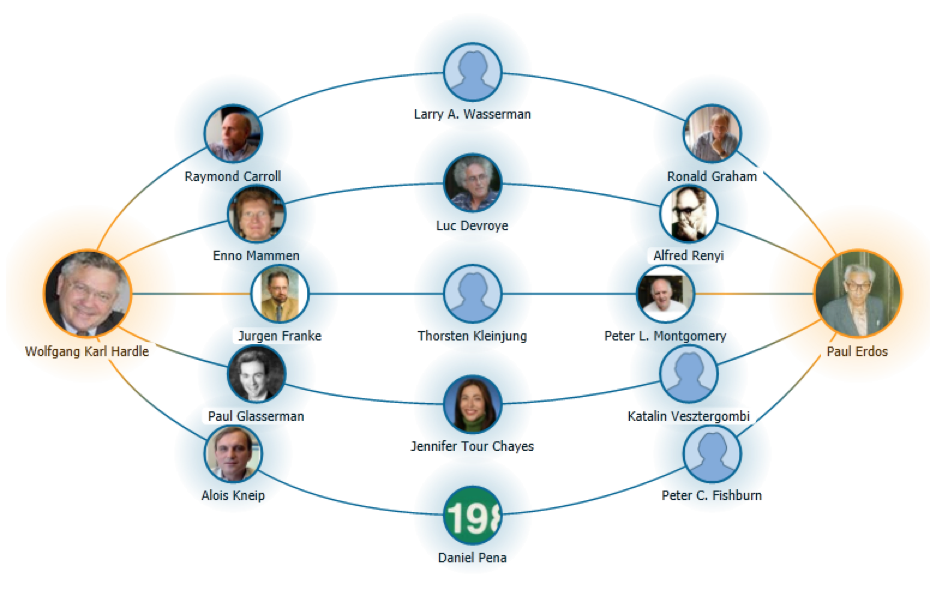
\includegraphics[scale=0.45]{figures/coauthorpath.png}
\caption{Coauthorship path of W.K. H\"ardle}
\bigskip
\scriptsize{
\href{http://academic.research.microsoft.com/VisualExplorer\#12530409\& 1112639}{Source: Microsoft Academic}}
\end{figure}
}

\frame{
\frametitle{A More Specific Coauthorship Graph}
\begin{figure}
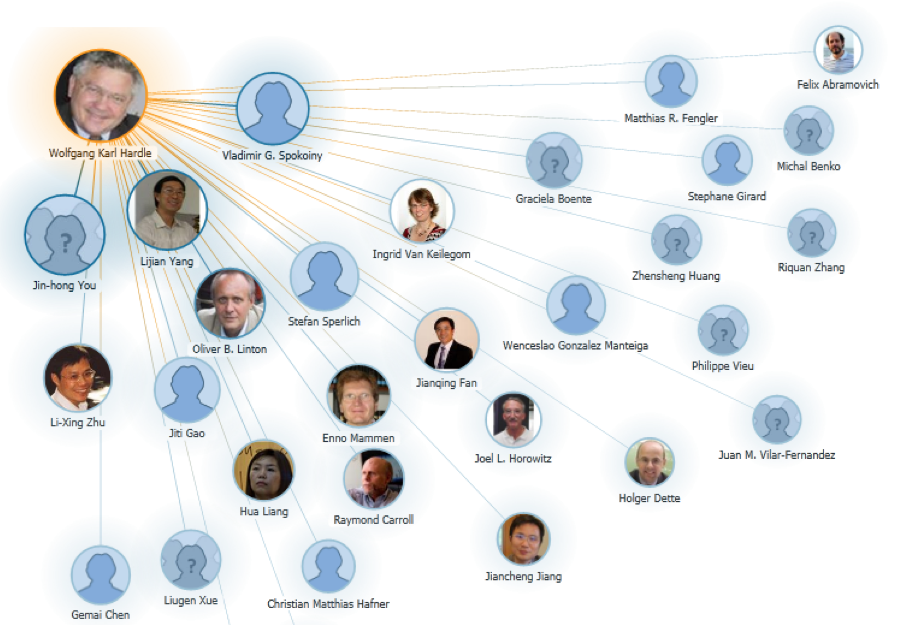
\includegraphics[scale=0.42]{figures/citationpath.png}
\caption{Citation path of W.K. H\"ardle}
\bigskip
\scriptsize{
\href{http://academic.research.microsoft.com/VisualExplorer\#12530409\& citation}{Source: Microsoft Academic}}
\end{figure}
}


\frame[plain]{
\frametitle{Outline}
\begin{enumerate}
\item Motivation \quad \checkmark
\item Definition
\item Relation to Adjacency Matrix
\item Network Centrality
\item Comparison of Various Centralities 
\end{enumerate}
}

\section{Definition}
\frame{
\frametitle{Network Structure}
$\mathcal{G}=(\mathcal{V},\mathcal{E})$ 
\bigskip{}
\begin{itemize}
\item vertices $\mathcal{V}$: each individual in your context
\bigskip
\item edges $\mathcal{E}$: linkages between every pair of vertices 
\end{itemize}
}

\section{Adjacency Matrix}
\frame{
\frametitle{Adjacency Matrix \& Network}
\color{isegreen}
\textbf{Example 1:} symmetric, unweighted adjacency matrix with 4 nodes 
\smallskip
\begin{columns}[onlytextwidth]
\begin{column}{0.5\textwidth}

$
A =
  \begin{bmatrix}
    0 & 1 & 0 & 0 \\
    1 & 0 & 1 & 1 \\
    0 & 1 & 0 & 0 \\
    0 & 1 & 0 & 0 \\
  \end{bmatrix}
$
\end{column}
\color{black}
\hspace*{0.2cm}\begin{column}{0.5\textwidth}
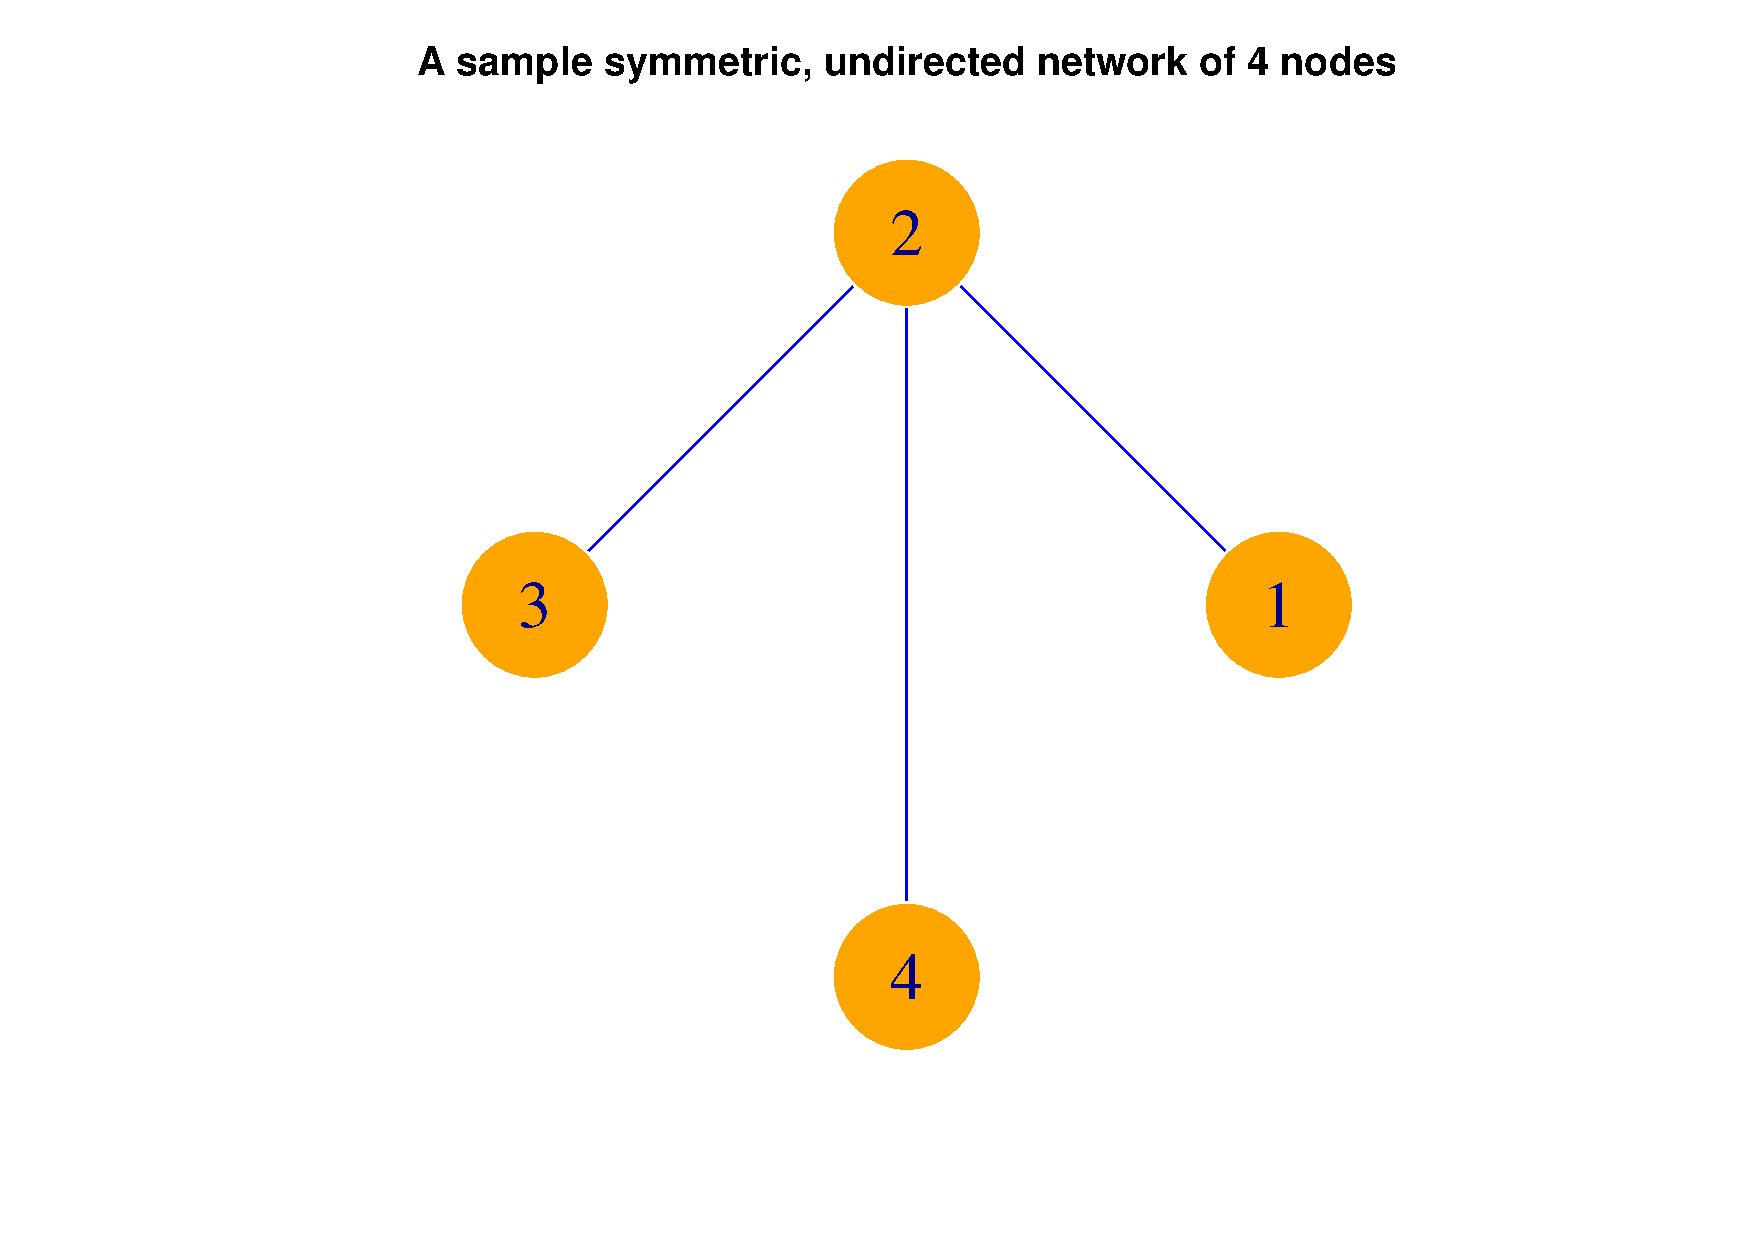
\includegraphics[scale=0.20]{figures/4nundirected.pdf}
\end{column}
\end{columns}
\href{https://github.com/QuantLet/METISNET/tree/master/METISNET-adjtonet}{\quantnet METISNET-adjtonet}
}


\frame{
\frametitle{Adjacency Matrix \& Network}
\color{isegreen}
\textbf{Example 2:} asymmetric, unweighted adjacency matrix with 4 nodes
\smallskip
\begin{columns}[onlytextwidth]
\begin{column}{0.5\textwidth}

$
A=
  \begin{bmatrix}
    0 & 0 & 1 & 0 \\
    0 & 0 & 1 & 0 \\
    0 & 1 & 0 & 0 \\
    1 & 0 & 1 & 0 \\
  \end{bmatrix}
$
\end{column}
\color{black}
\hspace*{0.2cm}\begin{column}{0.5\textwidth}
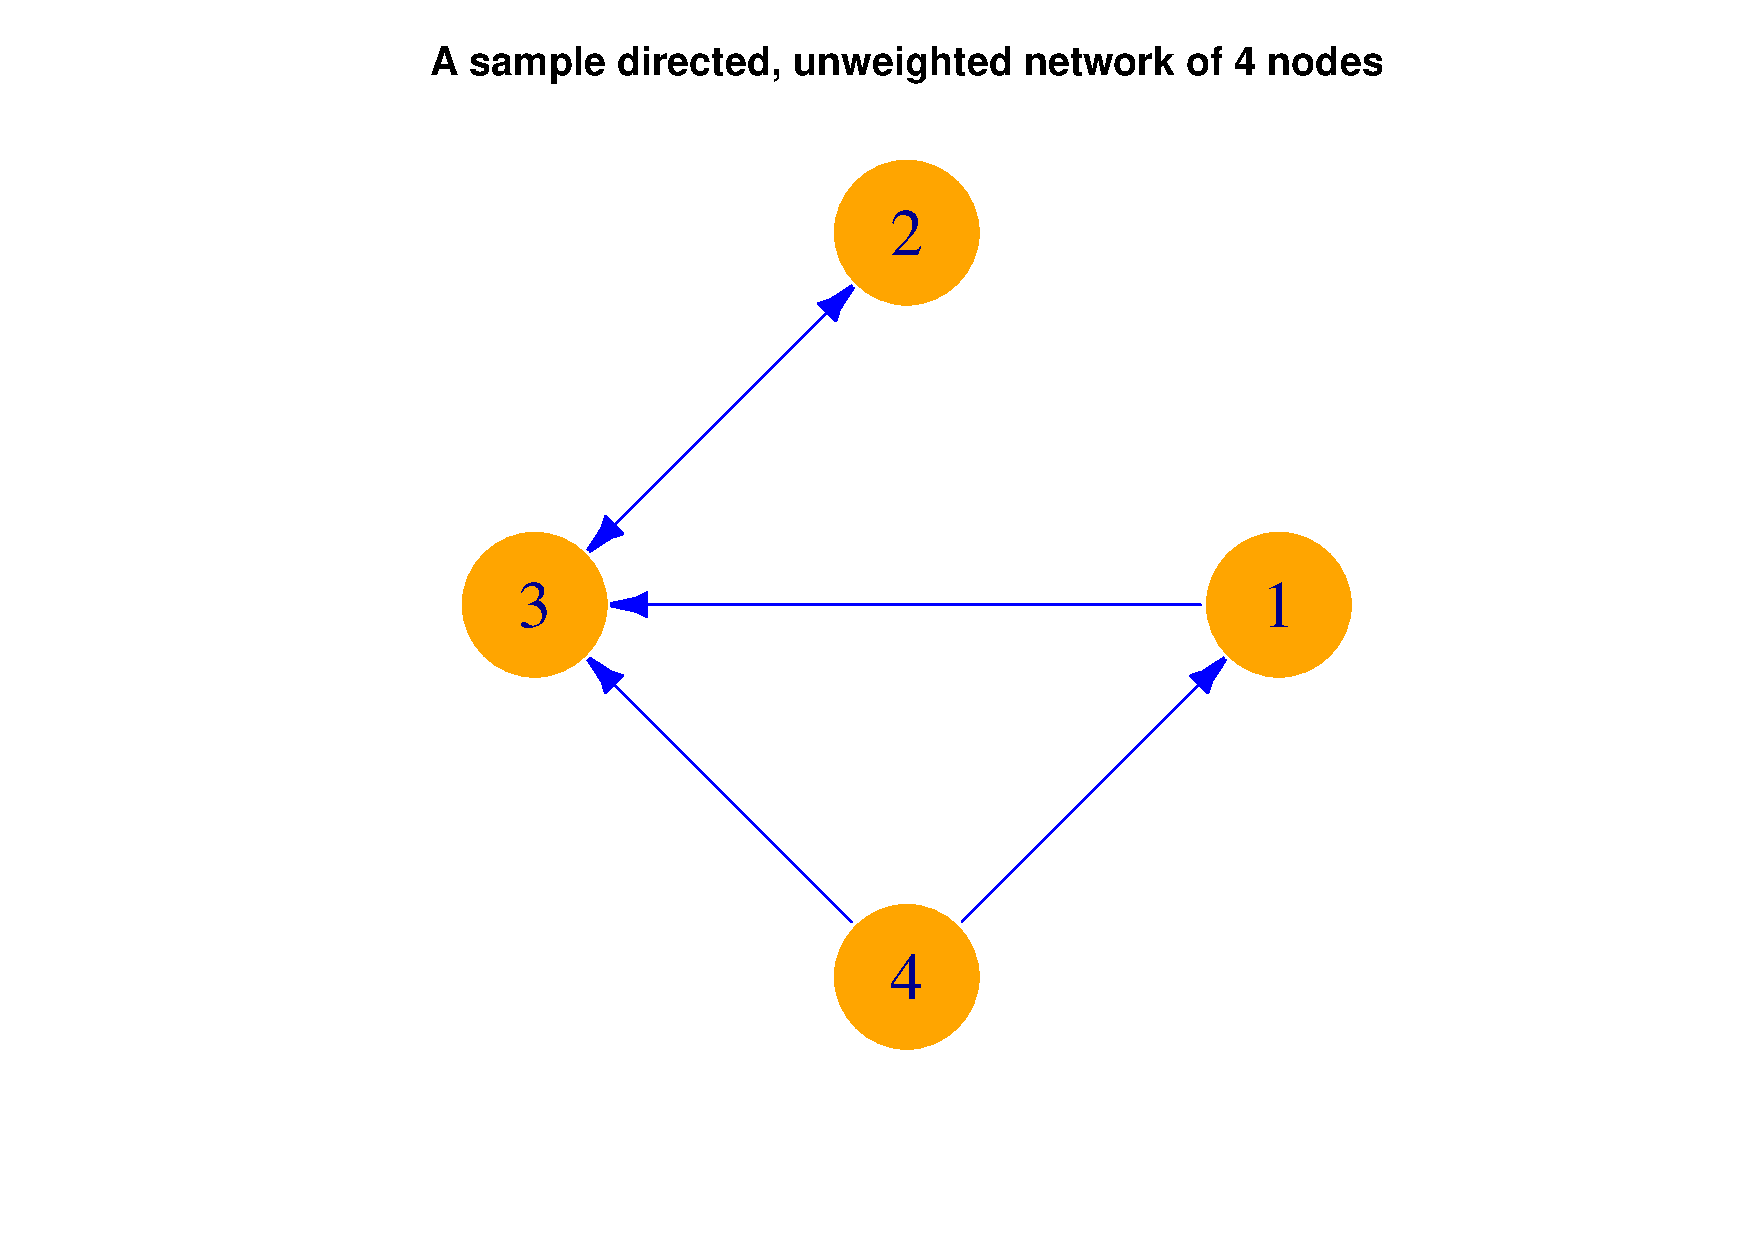
\includegraphics[scale=0.20]{figures/4ndirected.pdf}
\end{column}
\end{columns}
\href{https://github.com/QuantLet/METISNET/tree/master/METISNET-adjtonet}{\quantnet METISNET-adjtonet}
}


\frame{
\frametitle{Adjacency Matrix \& Network}
\color{isegreen}
\textbf{Example 3:} asymmetric, weighted adjacency matrix with 4 nodes
\smallskip
\begin{columns}[onlytextwidth]
\begin{column}{0.5\textwidth}

$
A=
  \begin{bmatrix}
    0 & 0.3 & 0.7 & 0 \\
    0 & 0 & 1 & 0 \\
    0 & 1 & 0 & 0 \\
    0.1 & 0 & 0.9 & 0 \\
  \end{bmatrix}
$
\end{column}
\color{black}
\hspace*{0.2cm}\begin{column}{0.5\textwidth}
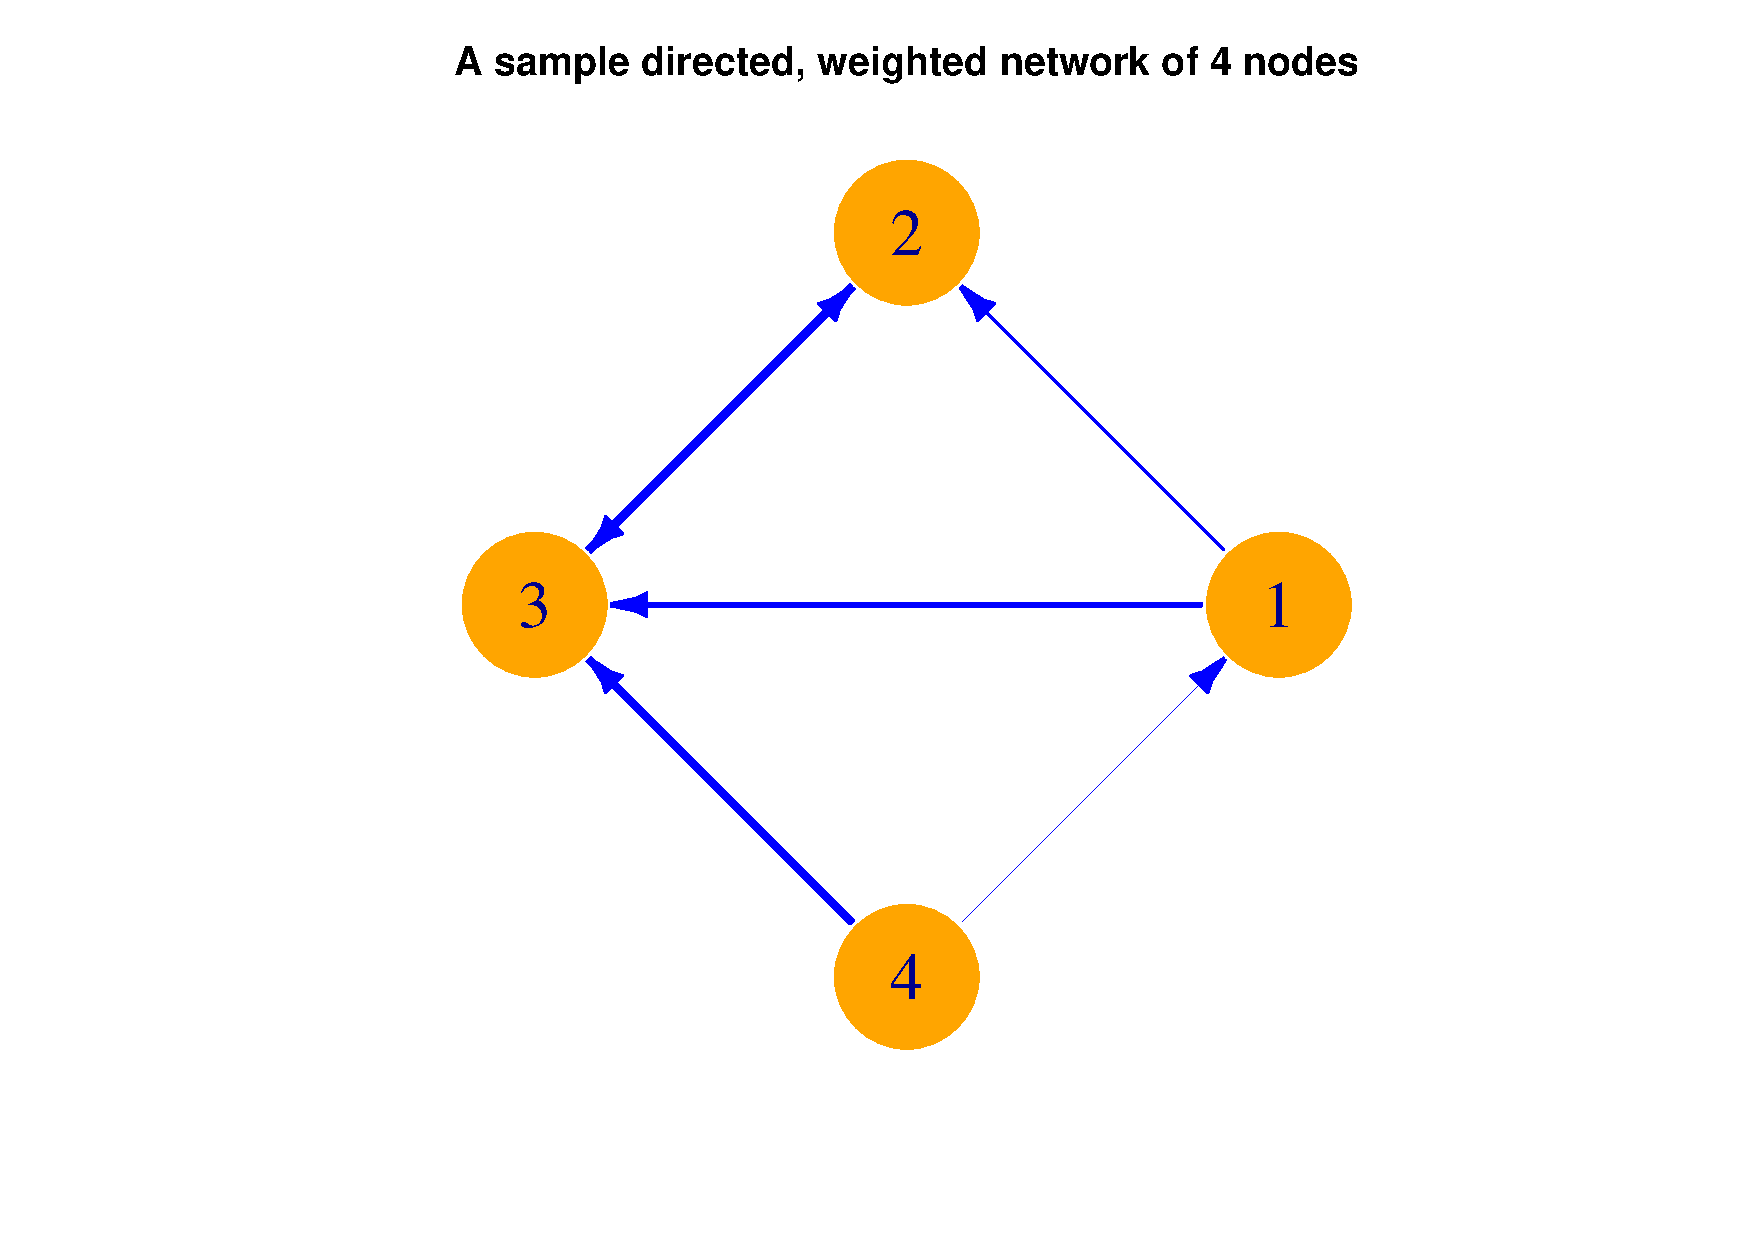
\includegraphics[scale=0.20]{figures/4ndirectedweighted.pdf}
\end{column}
\end{columns}
\href{https://github.com/QuantLet/METISNET/tree/master/METISNET-adjtonet}{\quantnet METISNET-adjtonet}
}

\section{Network Centrality}
%\subsection{Connectedness}
%\frame{
%\frametitle{Connectedness}
%\begin{itemize}
%\item To connectedness -- $C_{to}$
%\item From connectedness -- $C_{from}$
%\item Total connectedness -- $C_{total}$
%\end{itemize}
%}

%\frame{
%\frametitle{Connectedness}
%For an adjacency matrix $A = \{a_{ij}\}_{i,j=1}^n$ which denotes the network
%\begin{align*}
%C_{to,j} &= \sum_{i\neq j}a_{ij}, j = 1, 2, \ldots, n\\
%C_{from,j} &= \sum_{i\neq j}a_{ji},  j = 1, 2, \ldots, n\\
%C_{total} &= \frac{1}{n}\sum_{i,j=1}^{n}a_{ij}
%\end{align*} 
%}

\subsection{Centrality}
\frame{\frametitle{Network Centrality}
\begin{itemize}
\item Degree centrality
\item Closeness centrality
\item Betweenness centrality
\item Eigenvector centrality
\item Katz centrality
\item PageRank centrality
\item Percolation centrality
\item Cross-clique centrality
\item Freeman Centrality
\end{itemize}
}

\frame{
\frametitle{Degree Centrality}
For a network $\mathcal{G}=(\mathcal{V},\mathcal{E})$, degree centrality equals
\color{iseblue}
\begin{eqnarray*}
C_{D}(v) = \operatorname{deg}(v)
\end{eqnarray*}
\color{black}
where $\operatorname{deg}(v)$ denotes the total number of edges vertice $v$ has.\\
}


\frame{
\frametitle{Closeness Centrality}
For a network $\mathcal{G}=(\mathcal{V},\mathcal{E})$, closeness centrality equals
\color{iseblue}
\begin{eqnarray*}
C_C(v_1) = \frac{N-1}{\sum_{v_2}d(v_1,v_2)}
\end{eqnarray*}
\color{black}
\begin{itemize}
\item $N$: the total number of vertices
\item $d(v_1,v_2)$: distance between $v_1$ and $v_2$
\end{itemize}
}

\frame{
\frametitle{Betweenness Centrality}
For a network $\mathcal{G}=(\mathcal{V},\mathcal{E})$, betweenness centrality equals
\color{iseblue}
\begin{eqnarray*}
C_{B}(v) =\sum_{s\neq v\neq t \in \mathcal{V}} \frac{\sigma_{st}(v)}{\sigma_{st}}
\end{eqnarray*}
\color{black}
\begin{itemize}
\item $\sigma_{st}$: total amount of shortest paths from vertice $s$ to vertice $t$
\item $\sigma_{st}(v)$: total amount of shortest paths from vertice $s$ to vertice $t$ that passes through vertice $v$
\end{itemize}
}

\frame{
\frametitle{More about 'distance'}
\begin{itemize}
\item related to $C_{C}$ and $C_{B}$
\item the number of edges in the shortest connecting path (in the sense of edge number) -- unweighted
\item the real length of shortest connecting path (in the sense of real length)-- weighted
\item considered as a 'cost'
\end{itemize}
Example is given at the end of this talk : Minnesota Road Networks
}
 


\frame{
\frametitle{Eigenvector Centrality}
For a network $\mathcal{G}=(\mathcal{V},\mathcal{E})$, eigenvector centrality equals
\color{iseblue}
\begin{align*}
C_{E}(v) &=\frac{1}{\lambda}\sum_{t \in M(v)} C_{E}(t) = \frac{1}{\lambda} \sum_{t \in \mathcal{G}}a_{v,t} C_{E}(t)\\
\lambda C_{E} &= AC_{E}
\end{align*}
\color{black}
\begin{itemize}
\item $A=\{a_{v,t}\}_{v,t=1}^N$ is a 0-1 adjacency matrix
\item $\lambda$: maximum eigenvalue of $A$
\item $M(v)$: set of neighbors of $v$
\item $a_{v,t}$: the $vt_{th}$ element of $A$
\end{itemize}
}


\section{Comparison of Various Centralities}
\frame{
\frametitle{which is the central node?}
\color{isegreen}
\textbf{Example 4:} 
\smallskip
\begin{columns}[onlytextwidth]
\hspace{-2cm}
\begin{column}{0.5\textwidth}
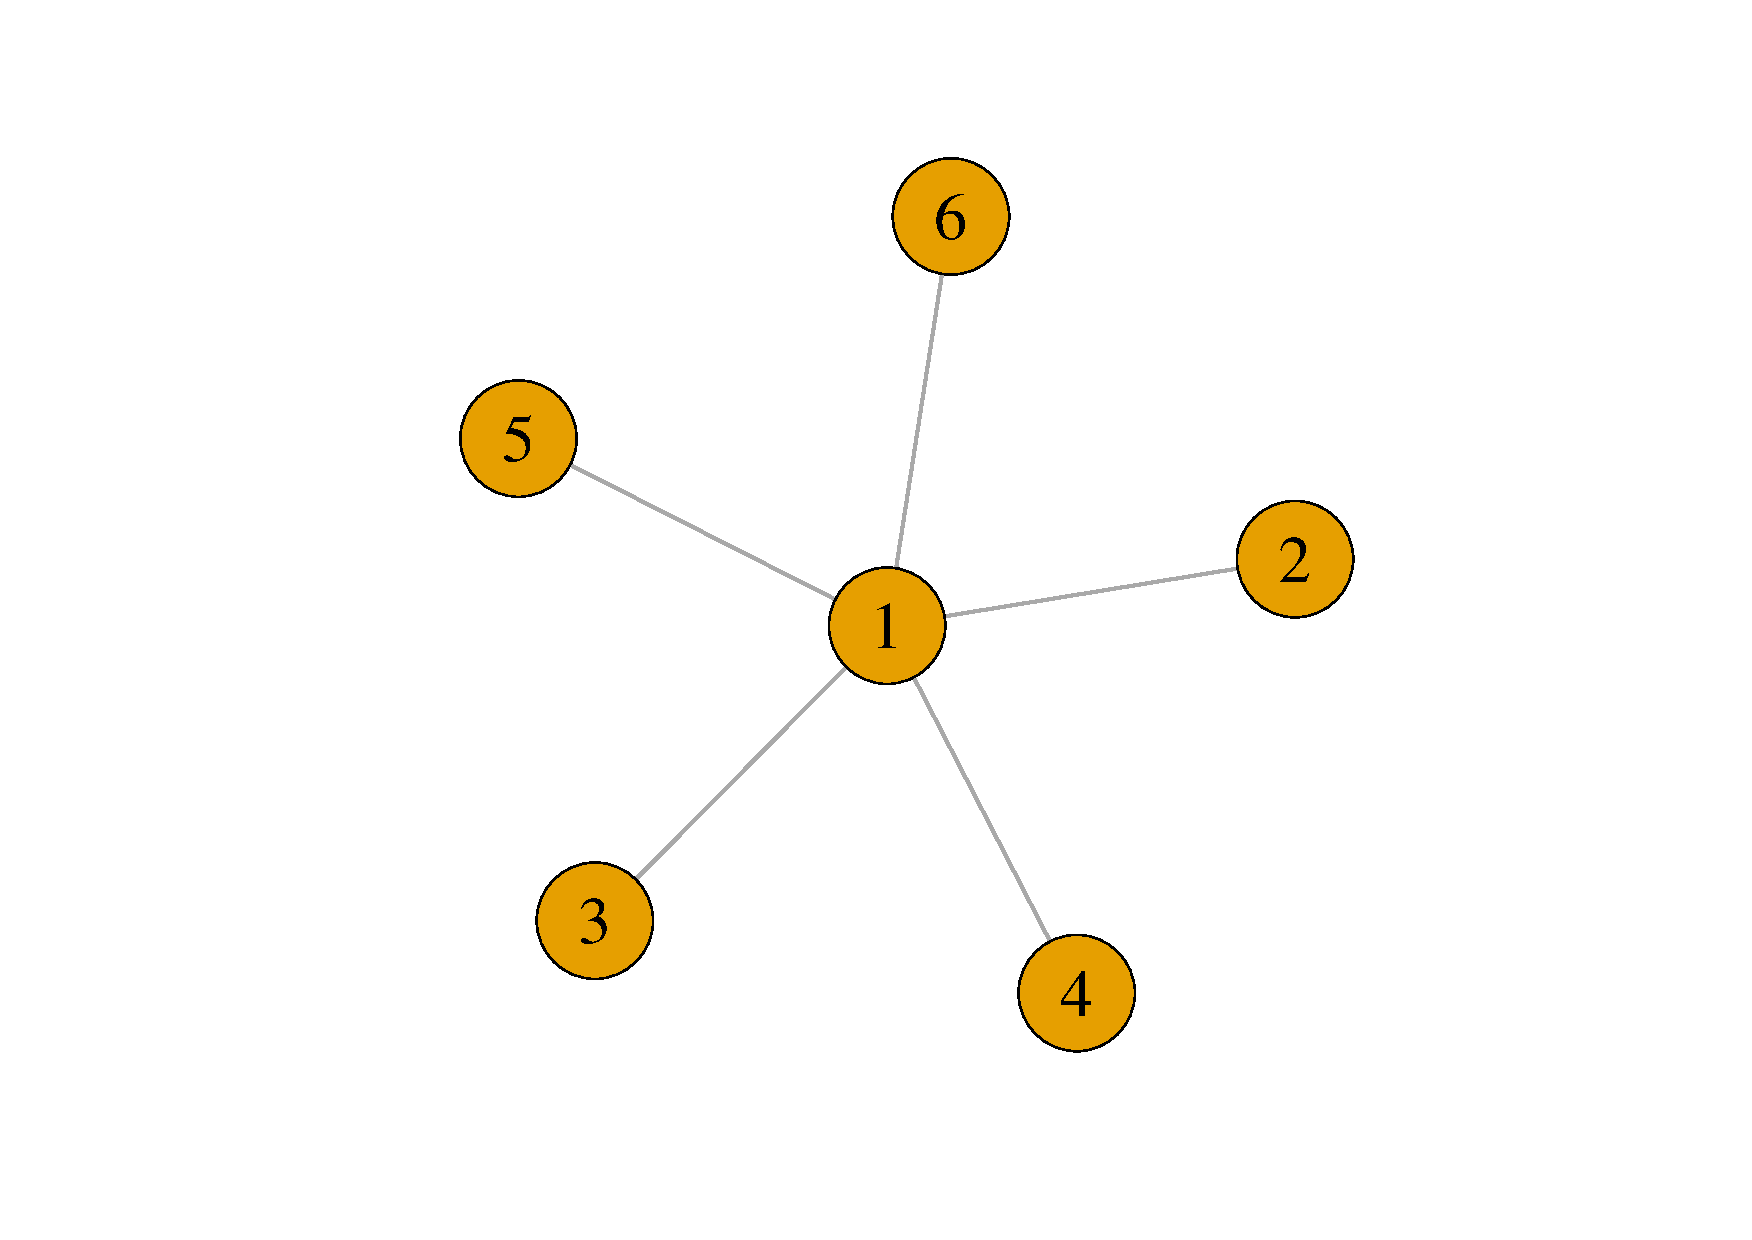
\includegraphics[scale=0.30]{figures/star.pdf}
\end{column}

\hspace*{0.2cm}\begin{column}{0.5\textwidth}
\begin{itemize}
\begin{small}
\color{isegreen}
\item $\mathbf{C_{D}(1) = 5}, C_{D}(2) = C_{D}(3) = C_{D}(4) = C_{D}(5) = C_{D}(6) = 1$
\item $\mathbf{C_{C}(1) = 1}, C_{C}(2) = C_{C}(3) = C_{C}(4) = C_{C}(5) = C_{C}(6) = 0.56$
\item $\mathbf{C_{B}(1) = 1}, C_{B}(2) = C_{B}(3) = C_{B}(4) = C_{B}(5) = C_{B}(6) = 0$
\item $\mathbf{C_{E}(1) = 0.71}, C_{E}(2) = C_{E}(3) = C_{E}(4) = C_{E}(5) = C_{E}(6) = 0.32$
\end{small}
\end{itemize}
\end{column}
\end{columns}
\color{black}
\vspace{-0.5cm}
\href{https://github.com/QuantLet/METISNET/tree/master/METISNET-adjtonet}{\quantnet METISNET-centralitymeasures}
}

%\frame{
%\frametitle{which is the central node?}
%\color{isegreen}
%\textbf{Example:} 
%\smallskip
%\begin{columns}[onlytextwidth]
%\begin{column}{0.5\textwidth}
%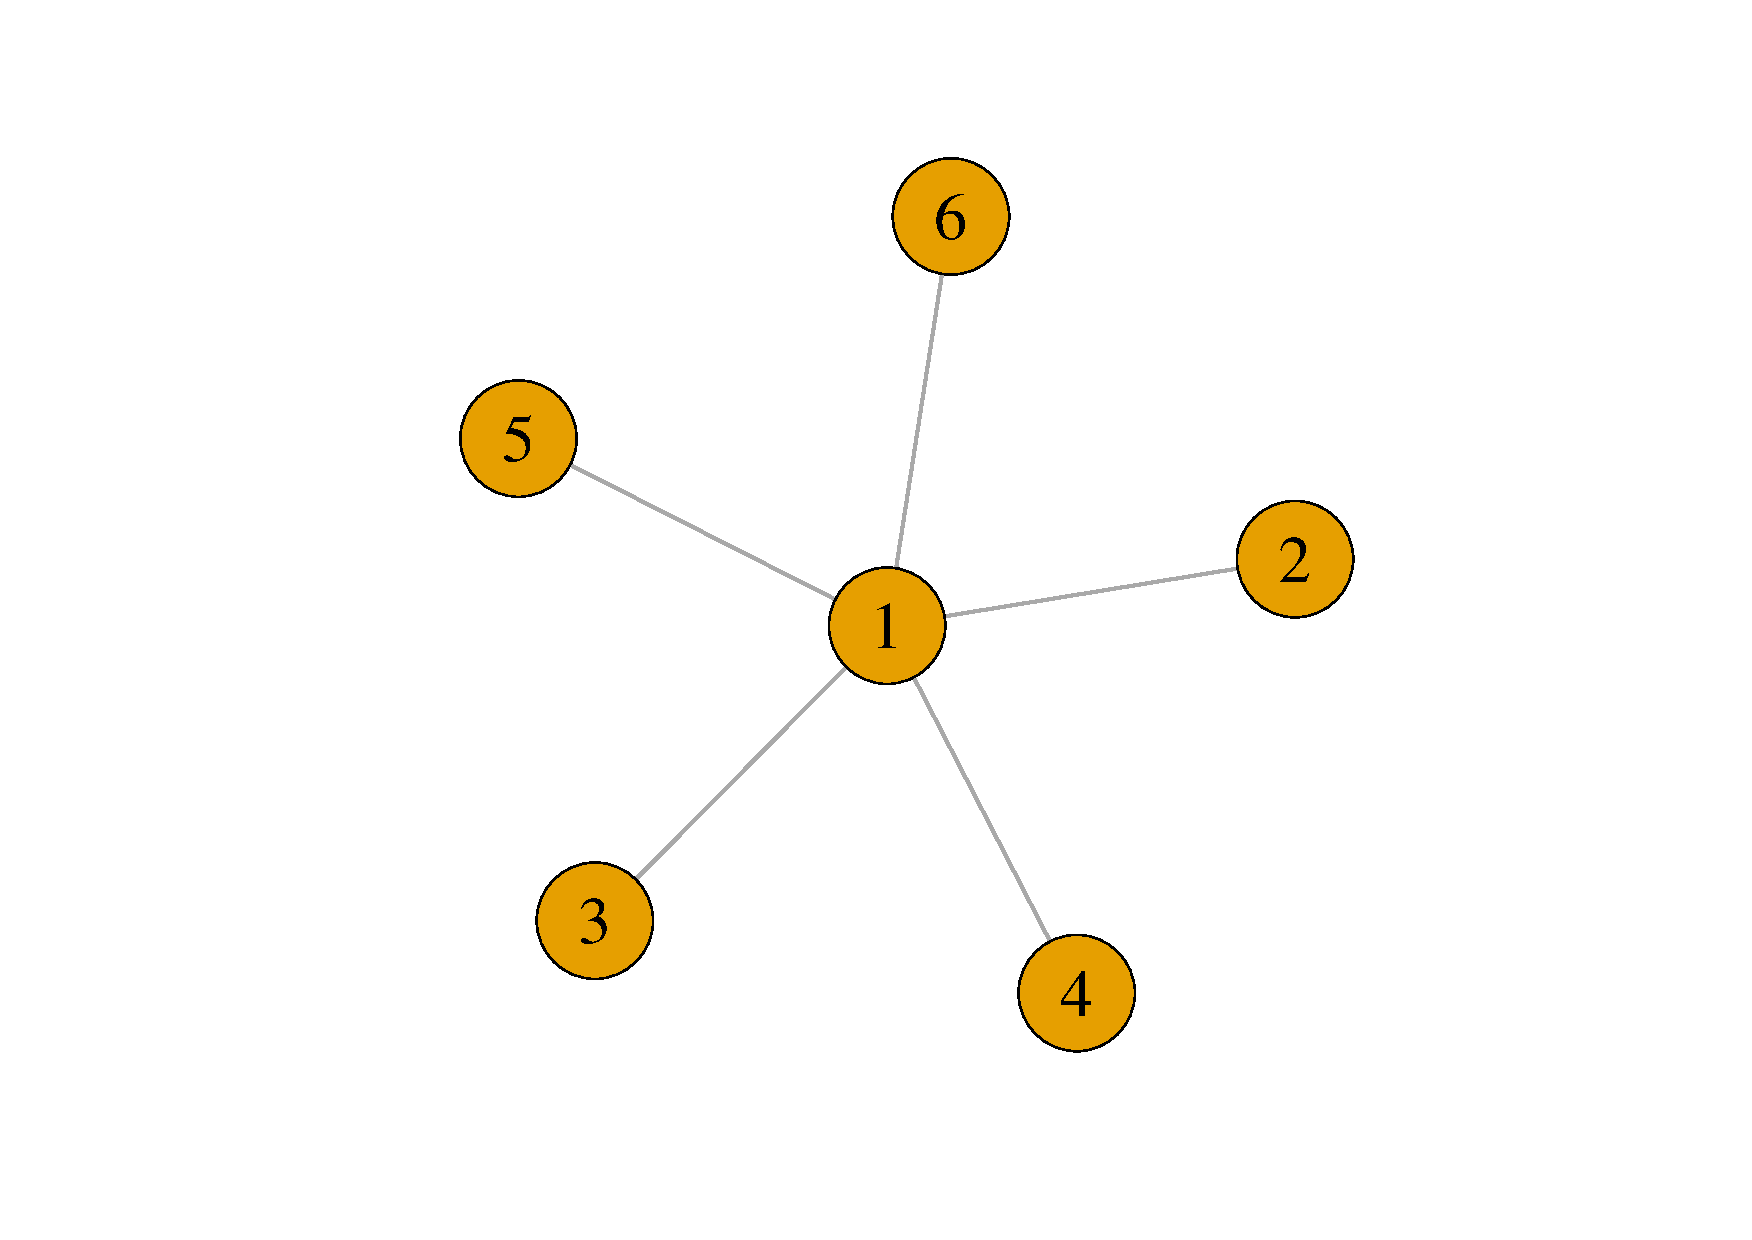
\includegraphics[scale=0.20]{figures/star.pdf}
%\end{column}
%\hspace*{0.2cm}\begin{column}{0.5\textwidth}
%\begin{itemize}
%\begin{tiny}
%\color{isegreen}
%\item degree centrality: node 1 has centrality 5, all others have centrality 1;
%\item closeness centrality: node 1 has centrality 1, all others have centrality 0.56;
%\item betweenness centrality: node 1 has centrality 1, all others have centrality 0;
%\item eigenvector centrality: node 1 has centrality 0.71, all others have centrality 0.32;
%\end{tiny}
%\end{itemize}
%\end{column}
%\end{columns}
%Conclusion: Node 1 is the central node by all centrality measures
%}

\frame{
\frametitle{which is the central node?}
\color{isegreen}
\textbf{Example 5:} 
\smallskip
\begin{columns}[onlytextwidth]
\hspace{-2cm}
\begin{column}{0.5\textwidth}
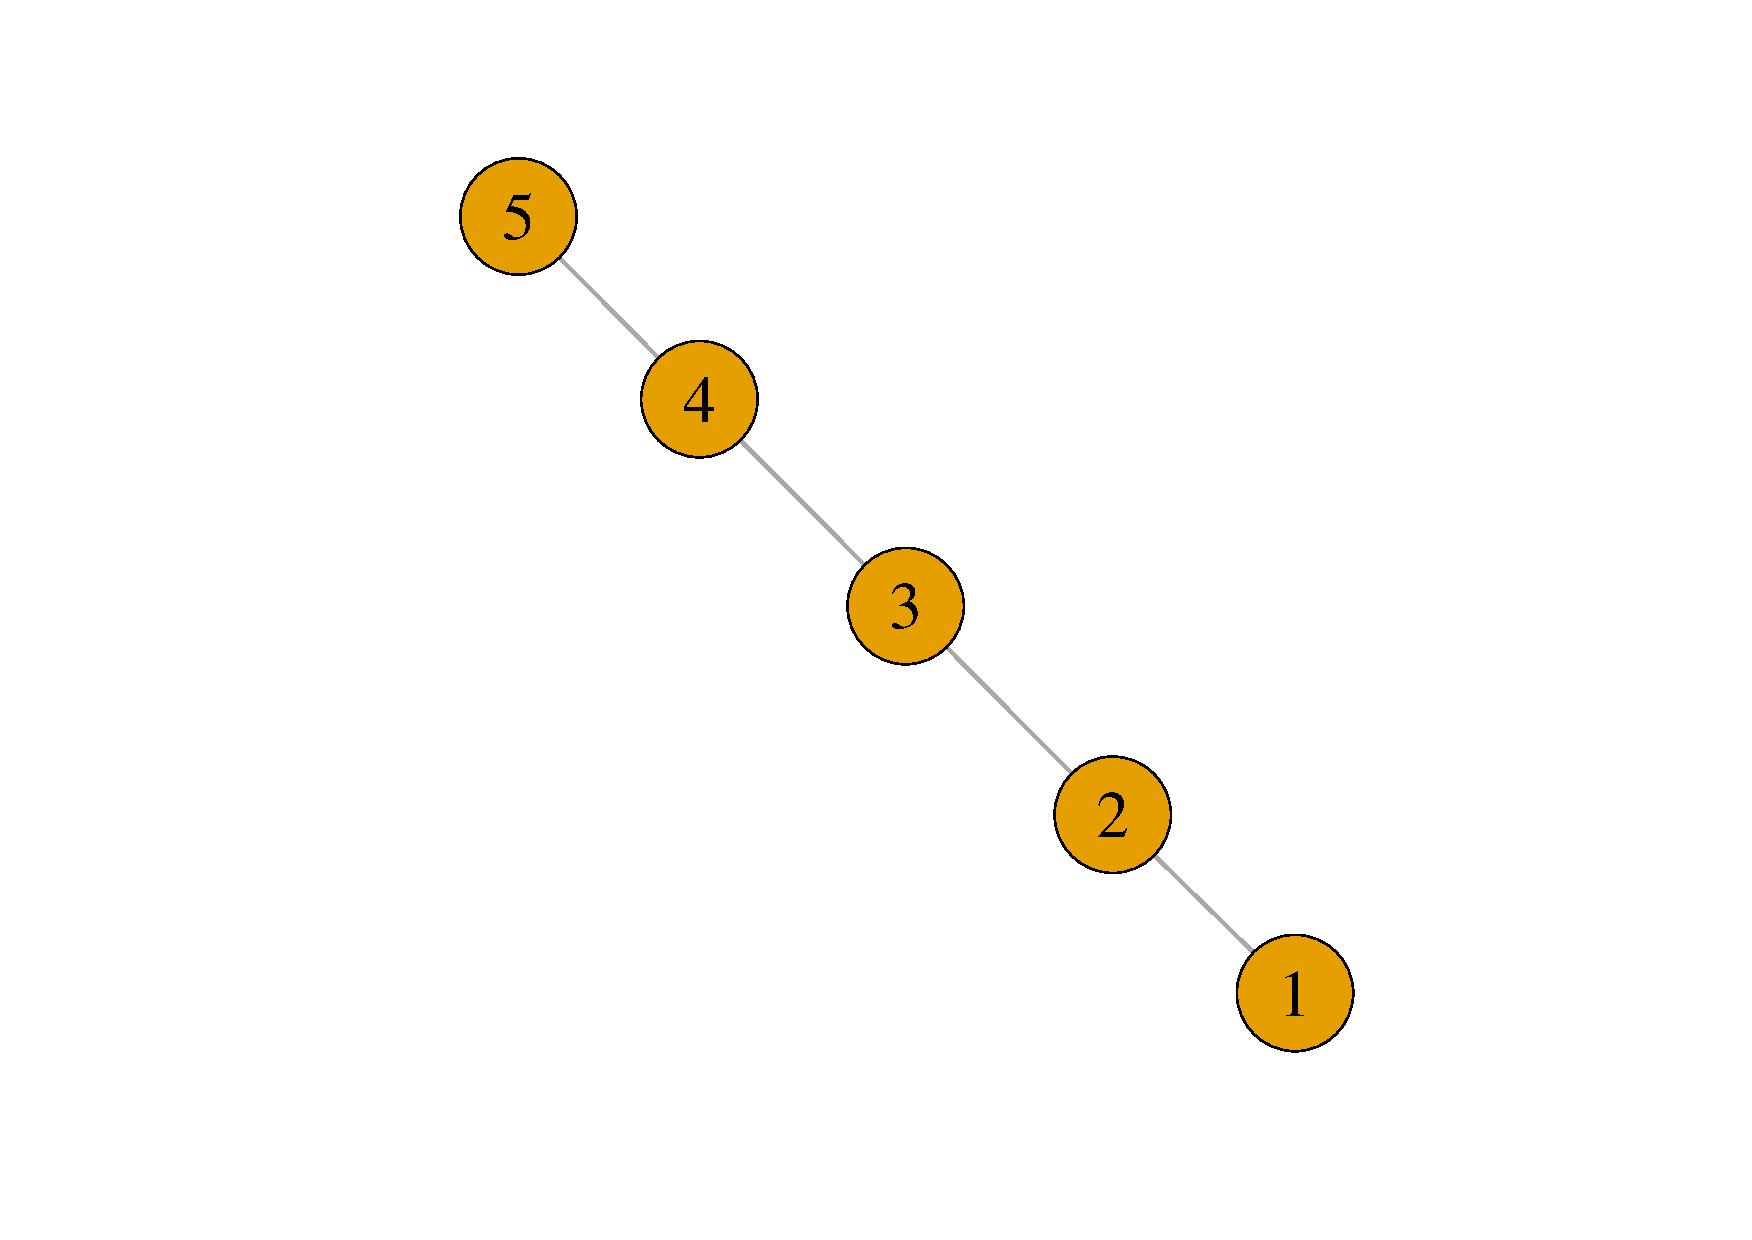
\includegraphics[scale=0.3]{figures/line.pdf}
\end{column}
\hspace*{0.2cm}\begin{column}{0.5\textwidth}
\begin{itemize}
\begin{small}
\color{isegreen}
\item $C_{D}(1) = C_{D}(5) = 1, \mathbf{C_{D}(2) = C_{D}(3) = C_{D}(4) = 2}$
\item $C_{C}(1) = C_{C}(5) = 0.4, C_{C}(2) = C_{C}(4) = 0.57, \mathbf{C_{C}(3) = 0.67}$
\item $C_{B}(1) = C_{B}(5) = 0, C_{B}(2) = C_{B}(4) = 0.50, \mathbf{C_{B}(3) = 0.67}$
\item $C_{E}(1) = C_{E}(5) = 0.29, C_{E}(2) = C_{E}(4) = 0.50, \mathbf{C_{B}(3) = 0.58}$
\end{small}
\end{itemize}
\end{column}
\end{columns}
\color{black}
\vspace{-0.8cm}
\href{https://github.com/QuantLet/METISNET/tree/master/METISNET-adjtonet}{\quantnet METISNET-centralitymeasures}
}

%\frame{
%\frametitle{which is the central node?}
%\color{isegreen}
%\textbf{Example:} 
%\smallskip
%\begin{columns}[onlytextwidth]
%\begin{column}{0.5\textwidth}
%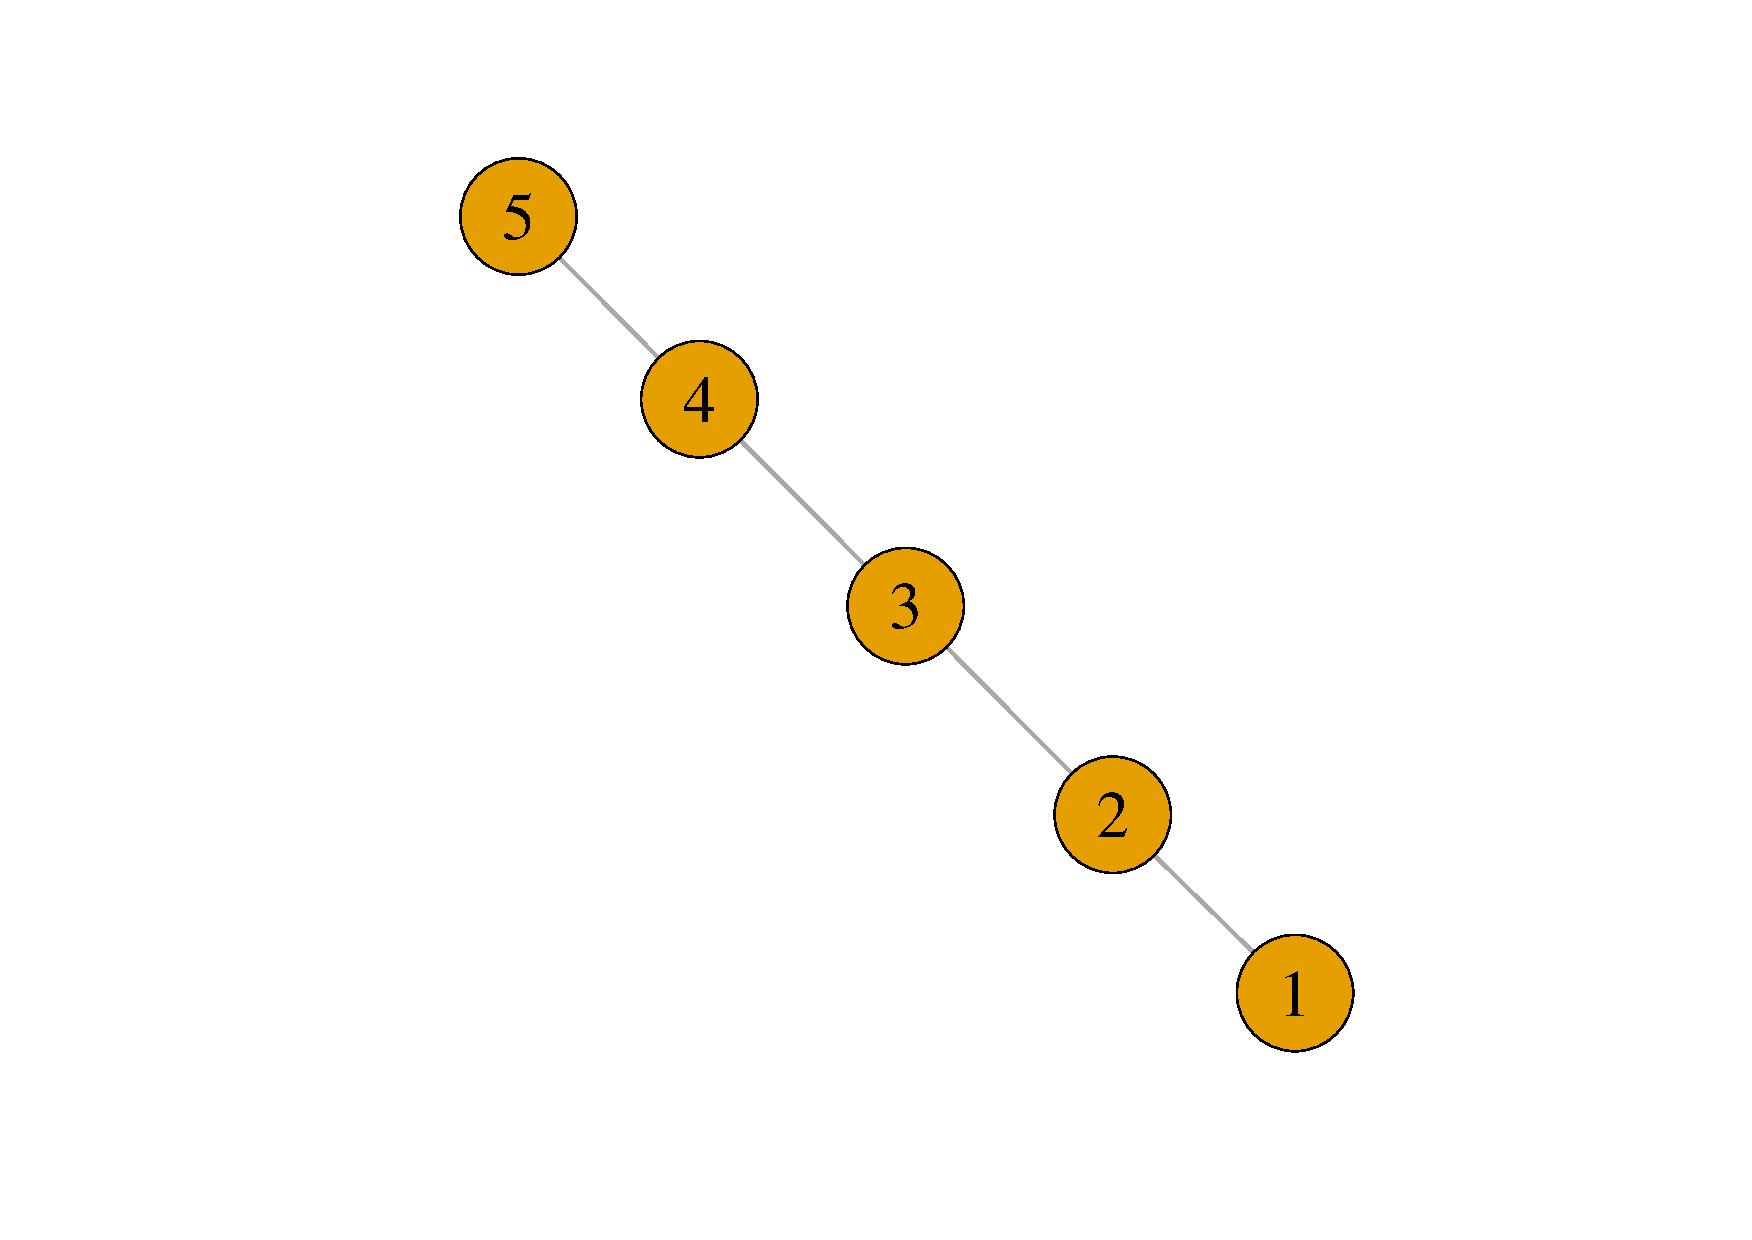
\includegraphics[scale=0.20]{figures/line.pdf}
%\end{column}
%\hspace*{0.2cm}\begin{column}{0.5\textwidth}
%\begin{itemize}
%\begin{tiny}
%\color{isegreen}
%\item degree centrality: node 1 and node 5 have centrality 1, all others have centrality 2;
%\item closeness centrality: node 1 and node 5 have centrality 0.4, node 2 and node 4 have centrality 0.57, node 3 has centrality 0.67;
%\item betweenness centrality: node 1 and node 5 have centrality 0, node 2 and node 4 have centrality 0.50, node 3 has centrality 0.67;
%\item eigenvector centrality: node 1 and node 5 have centrality 0.29, node 2 and node 4 have centrality 0.50, node 3 has centrality 0.58;
%\end{tiny}
%\end{itemize}
%\end{column}
%\end{columns}
%Conclusion: Node 3 is the central node by all centrality measures
%}

\frame{
\frametitle{which is the central node?}
\color{isegreen}
\textbf{Example 6:} 
\smallskip
\begin{columns}[onlytextwidth]
\hspace{-2cm}
\begin{column}{0.5\textwidth}
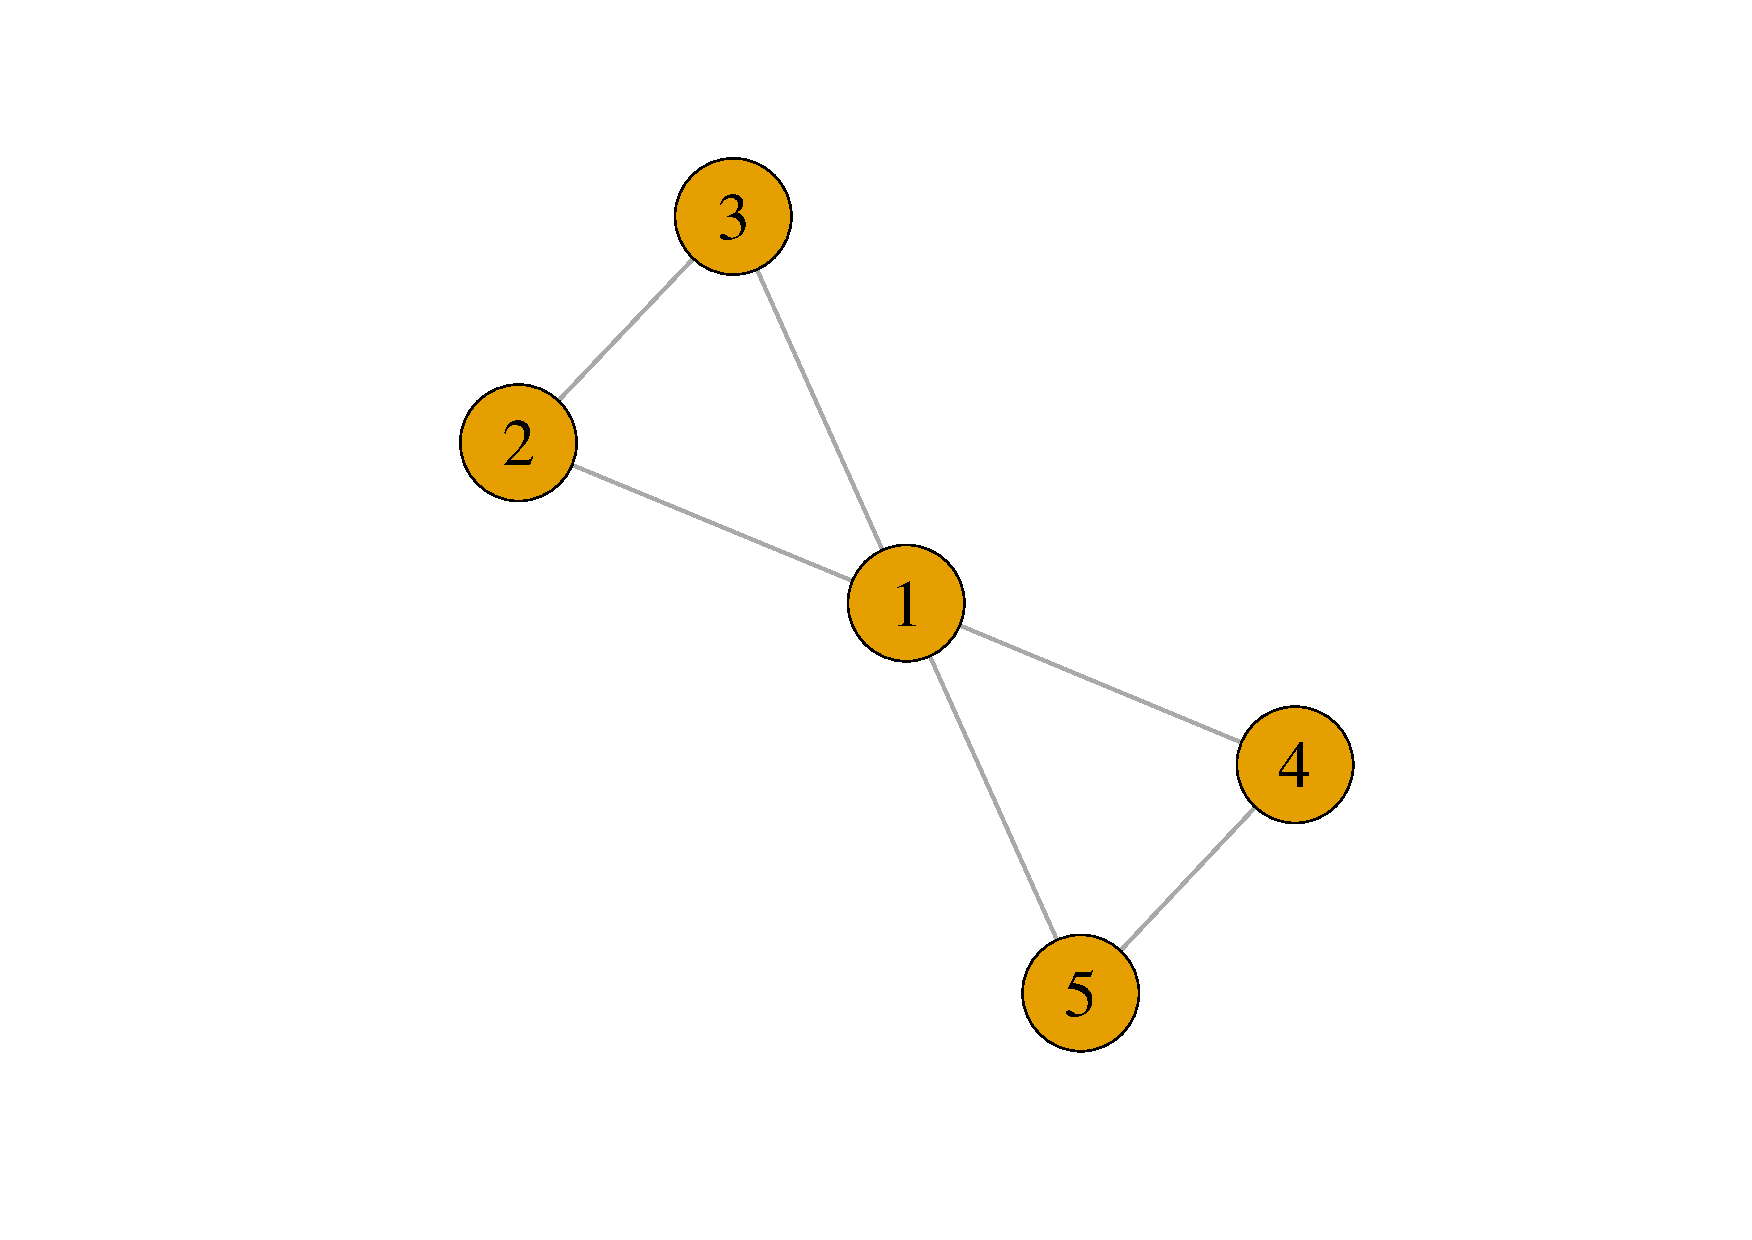
\includegraphics[scale=0.3]{figures/fork.pdf}
\end{column}
\hspace*{0.2cm}\begin{column}{0.5\textwidth}
\begin{itemize}
\begin{small}
\color{isegreen}
\item $\mathbf{C_{D}(1) = 4}, C_{D}(2) = C_{D}(3) = C_{D}(4) = C_{D}(5)= 2$
\item $\mathbf{C_{C}(1) = 1}, C_{C}(2) = C_{C}(3) = C_{C}(4) = C_{C}(5)= 0.67$
\item $\mathbf{C_{B}(1) = 0.67}, C_{B}(2) = C_{B}(3) = C_{B}(4) = C_{B}(5)= 0$
\item $\mathbf{C_{E}(1) = 0.62}, C_{E}(2) = C_{E}(3) = C_{E}(4) = C_{E}(5)= 0.39$
\end{small}
\end{itemize}
\end{column}
\end{columns}
\color{black}
\vspace{-0.8cm}
\href{https://github.com/QuantLet/METISNET/tree/master/METISNET-adjtonet}{\quantnet METISNET-centralitymeasures}
}

%\frame{
%\frametitle{which is the central node?}
%\color{isegreen}
%\textbf{Example:} 
%\smallskip
%\begin{columns}[onlytextwidth]
%\begin{column}{0.5\textwidth}
%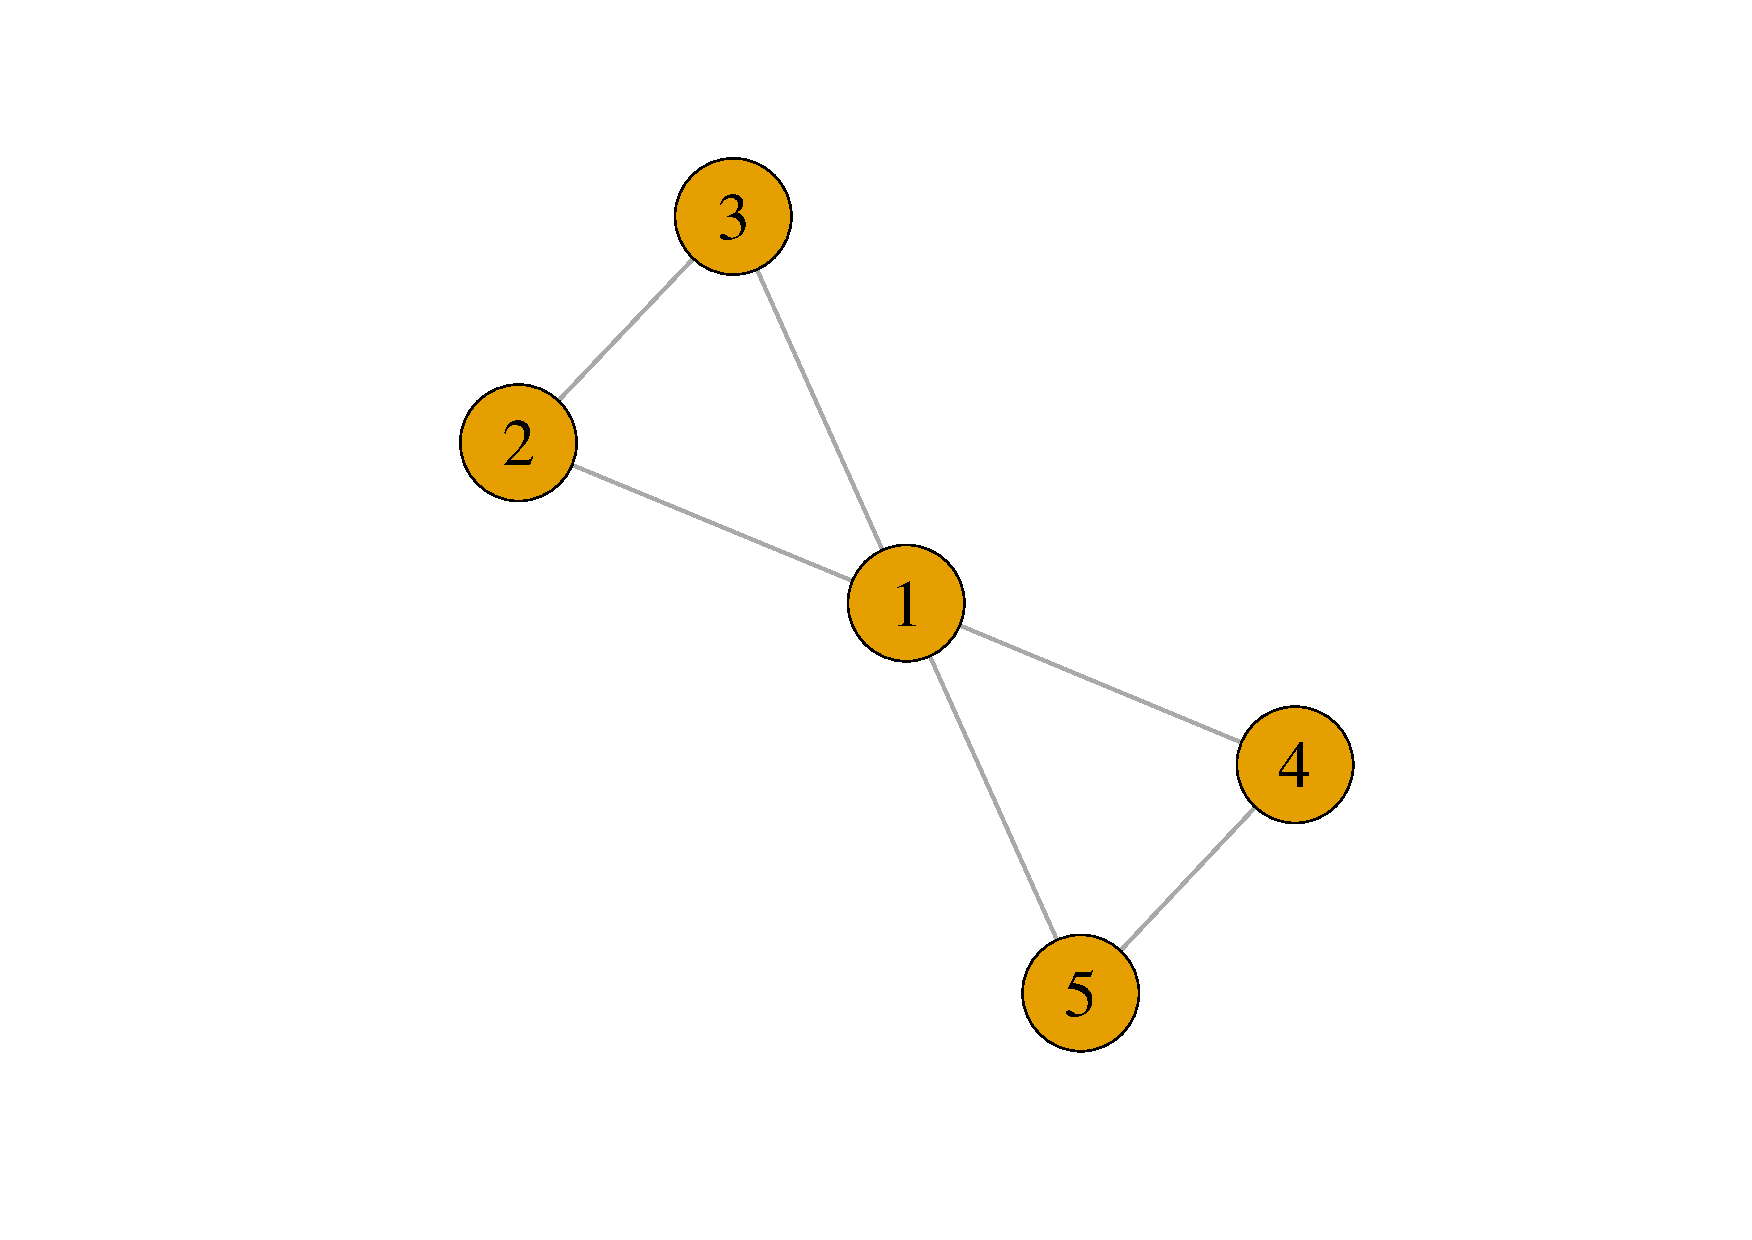
\includegraphics[scale=0.20]{figures/fork.pdf}
%\end{column}
%\hspace*{0.2cm}\begin{column}{0.5\textwidth}
%\begin{itemize}
%\begin{tiny}
%\color{isegreen}
%\item degree centrality: node 1 has centrality 4, all others have centrality 2;
%\item closeness centrality: node 1 has centrality 1, all others have centrality 0.67;
%\item betweenness centrality: node 1 has centrality 0.67, all others have centrality 0;
%\item eigenvector centrality: node 1 has centrality 0.62, all others have centrality 0.39;
%\end{tiny}
%\end{itemize}
%\end{column}
%\end{columns}
%Conclusion: Node 1 is the central node by all centrality measures
%}

\frame{
\frametitle{which is the central node?}
\color{isegreen}
\textbf{Example 7:}
\smallskip
\begin{columns}[onlytextwidth]
\hspace{-2cm}
\begin{column}{0.5\textwidth}
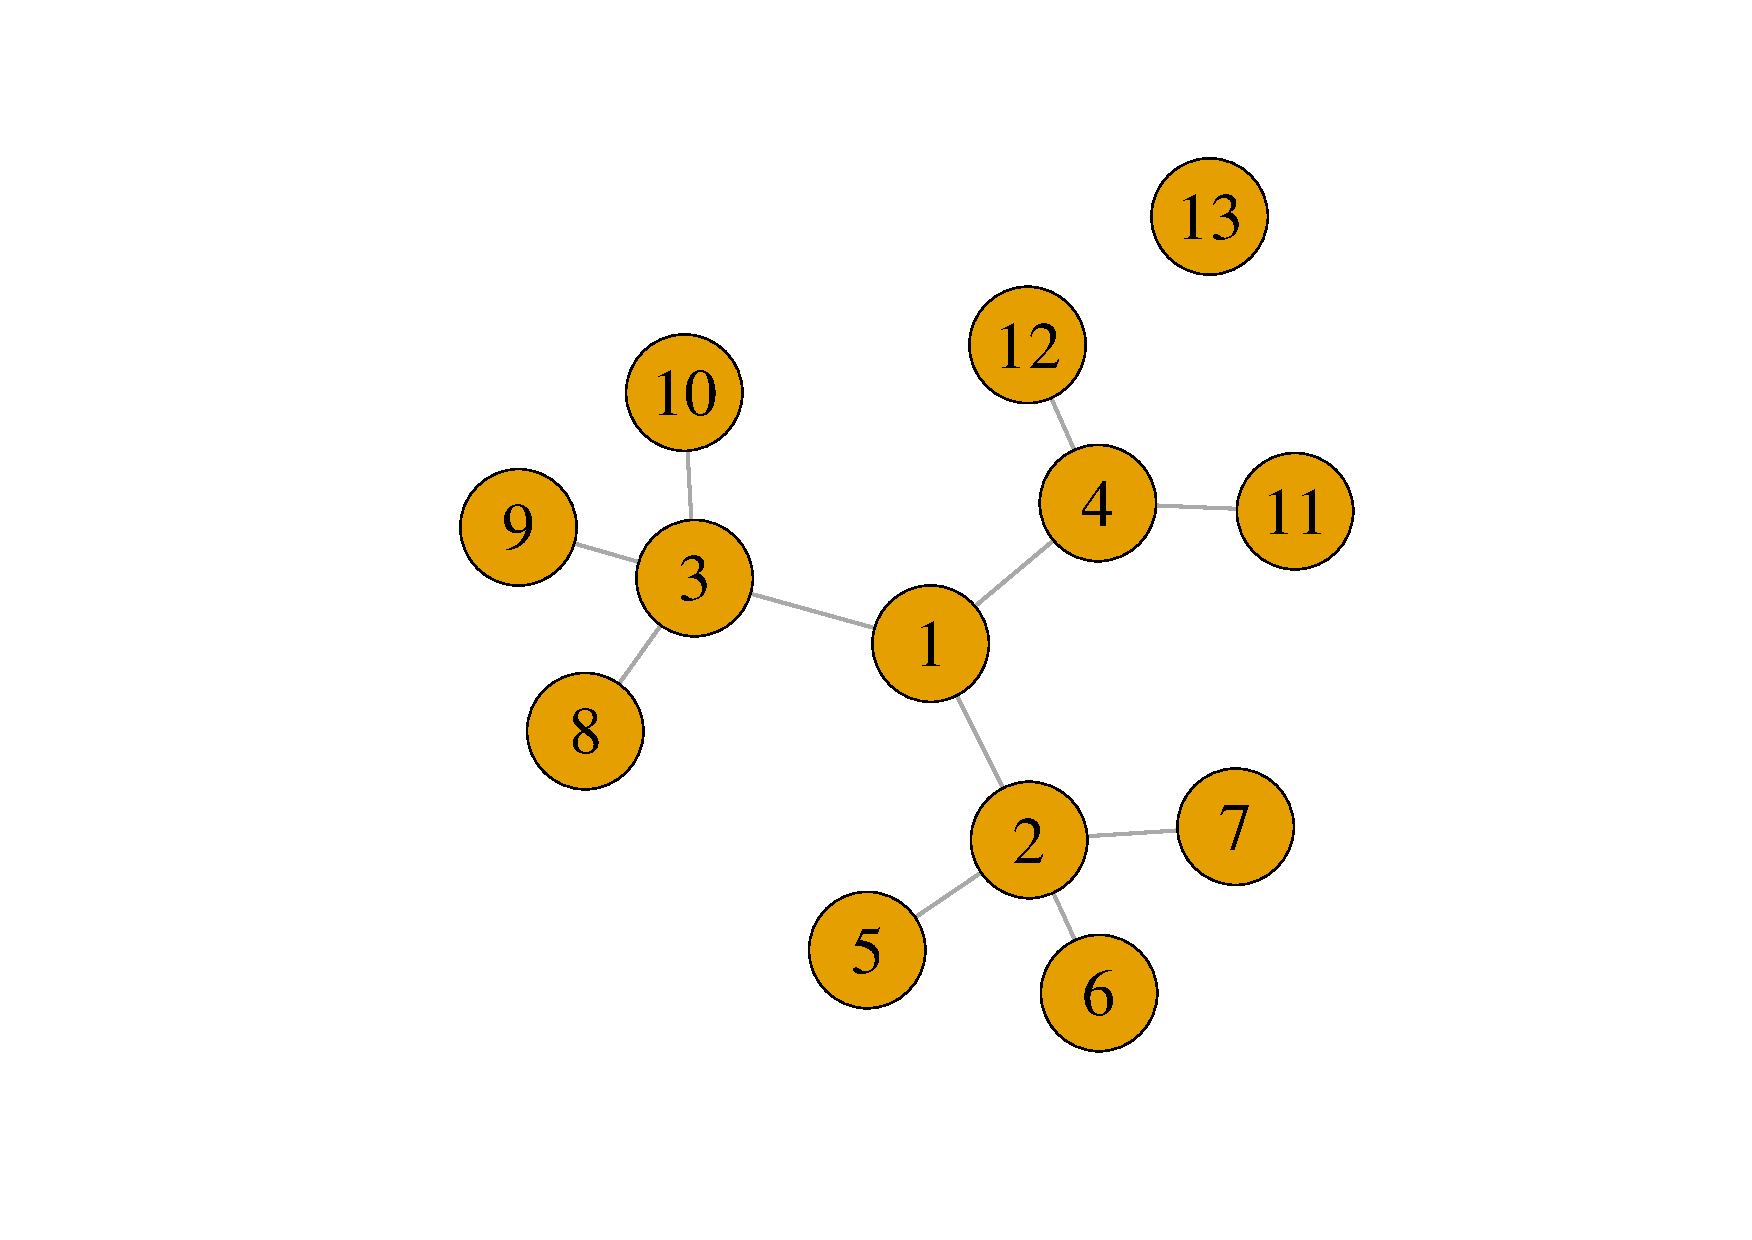
\includegraphics[scale=0.3]{figures/conteg.pdf}
\end{column}
\hspace*{0.2cm}\begin{column}{0.5\textwidth}
\begin{itemize}
\begin{small}
\color{isegreen}
\item $C_{D}(1) = C_{D}(4) = 3, \mathbf{C_{D}(2) = C_{D}(3) = 4}$
\item $\mathbf{C_{C}(1) = 0.63}, C_{C}(2) = C_{C}(3) = 0.52, C_{C}(4) = 0.48$
\item $\mathbf{C_{B}(1) = 0.61}, C_{B}(2) = C_{B}(3) = 0.36, C_{B}(4) = 0.27$
\item $\mathbf{C_{E}(1) = 0.51}, C_{E}(2) = C_{E}(3) = 0.44, C_{E}(4) = 0.33$
\end{small}
\end{itemize}
\end{column}
\end{columns}
\color{black}
\vspace{-1cm}
\href{https://github.com/QuantLet/METISNET/tree/master/METISNET-adjtonet}{\quantnet METISNET-centralitymeasures}
}

%\frame{
%\frametitle{which is the central node?}
%\color{isegreen}
%\textbf{Example:}
%\smallskip
%\begin{columns}[onlytextwidth]
%\begin{column}{0.5\textwidth}
%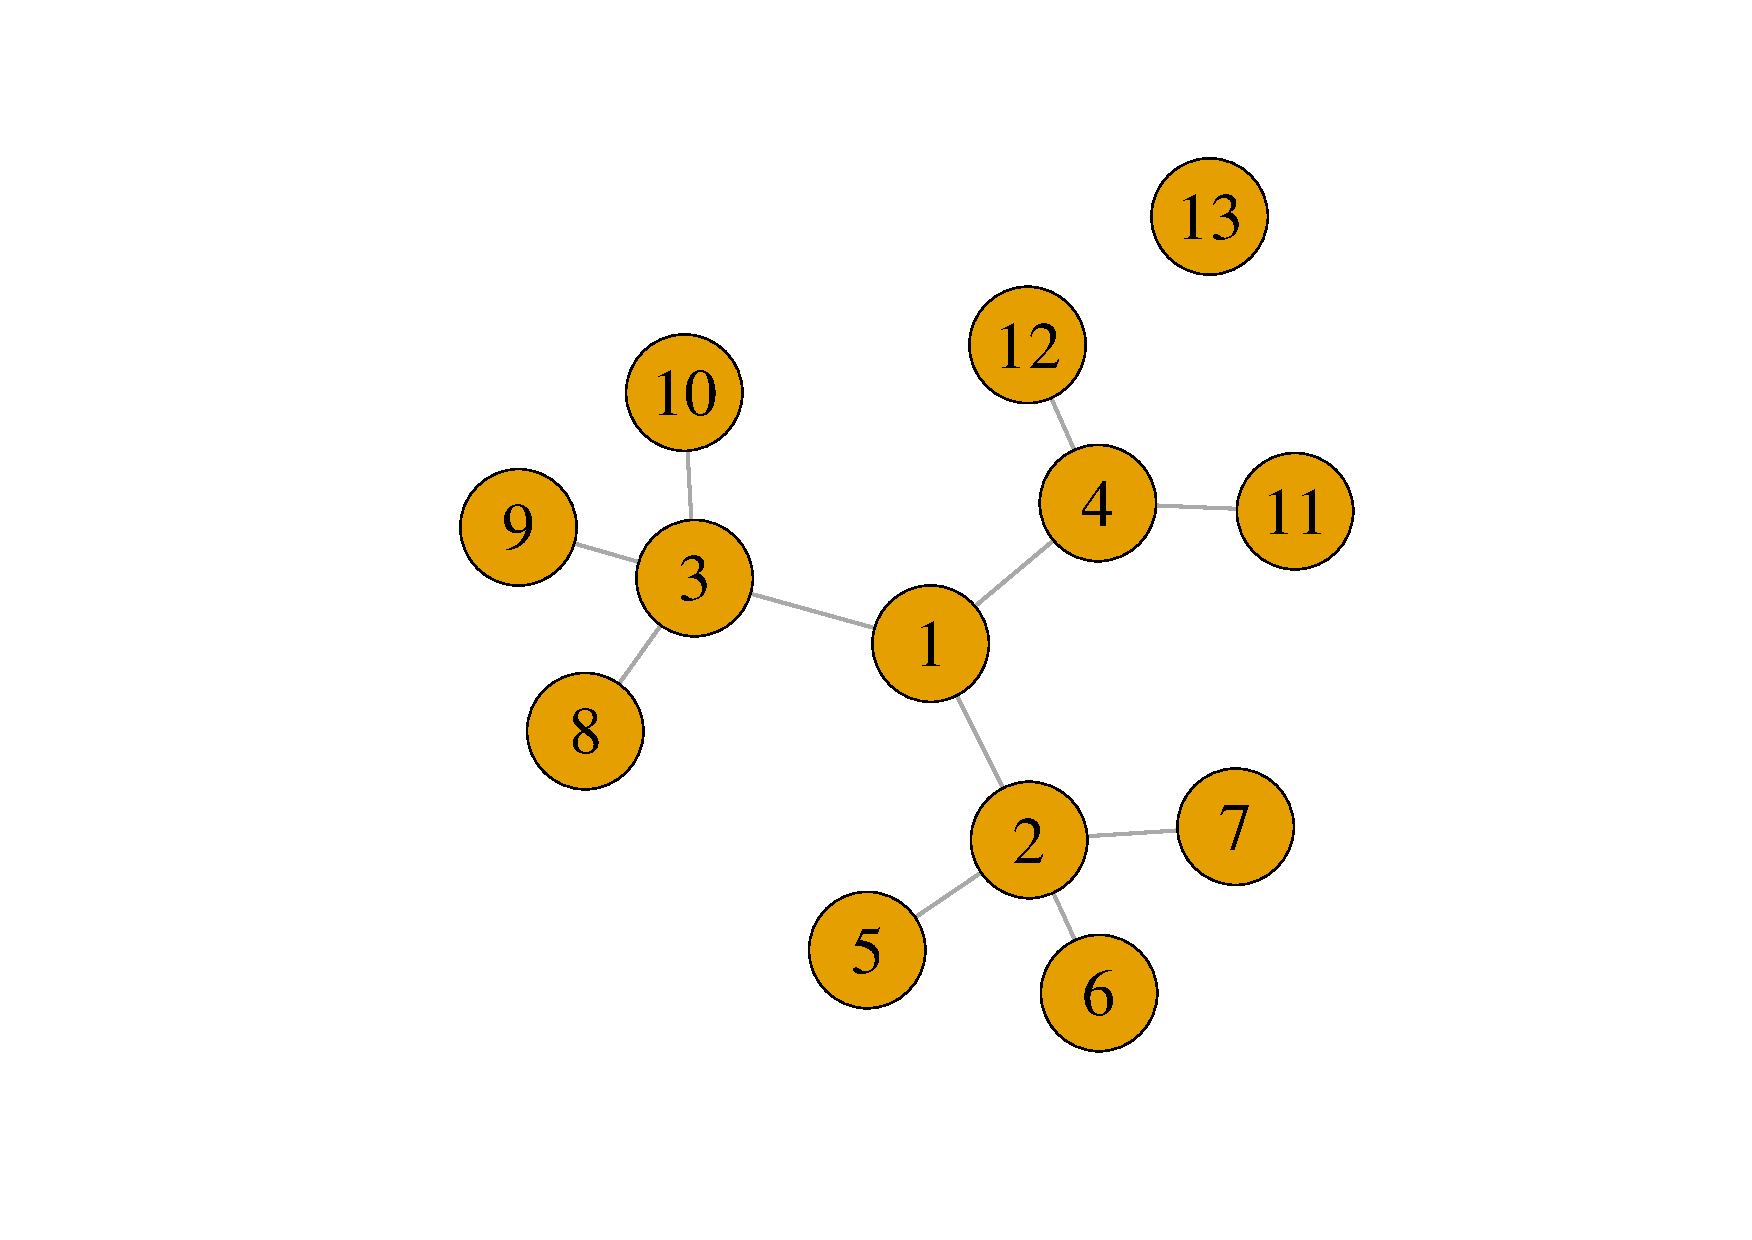
\includegraphics[scale=0.20]{figures/conteg.pdf}
%\end{column}
%\hspace*{0.2cm}\begin{column}{0.5\textwidth}
%\begin{itemize}
%\begin{tiny}
%\color{isegreen}
%\item degree centrality: node 1 has centrality 3, node 2 and 3 have centrality 4, node 4 has centrality 3;
%\item closeness centrality: node 1 has centrality 0.63, node 2 and 3 have centrality 0.52, node 4 has centrality 0.48;
%\item betweenness centrality: node 1 has centrality 0.61, node 2 and 3 have centrality 0.36, node 4 has centrality 0.27;
%\item eigenvector centrality: node 1 has centrality 0.51, node 2 and 3 have centrality 0.44, node 4 has centrality 0.33;
%\end{tiny}
%\end{itemize}
%\end{column}
%\end{columns}
%Conclusion: Node 1 is the central node by all centrality measures but degree centrality;
%Node 2 and 3 are central nodes by degree centrality
%}
%

\frame{
\frametitle{Minnesota Road Networks}
\begin{itemize}
\item Minnesota Road Net data \textcolor{purple}{minnesota.mat} is avaiable in Matlab R2016b and later versions
\item Minnesota State of United States
\item The data contains a $G$ object which is a combination of Nodes (Coordinates of locations) and Edges (roads between each pair of nodes)
\end{itemize}
}

\frame{
\frametitle{Minnesota Road Networks}
\begin{figure}
\begin{tabular}{cc}
\subfloat{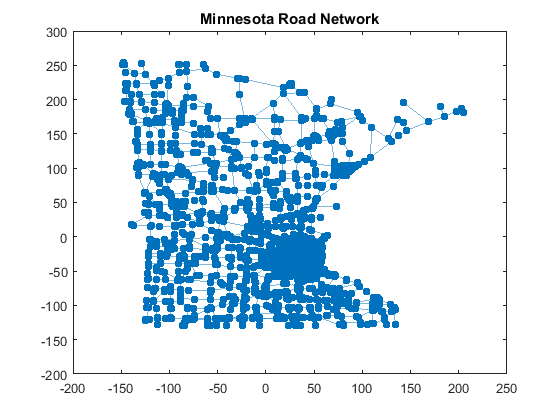
\includegraphics[scale=0.35]{figures/minnesotaroadnet.png}}
&\subfloat{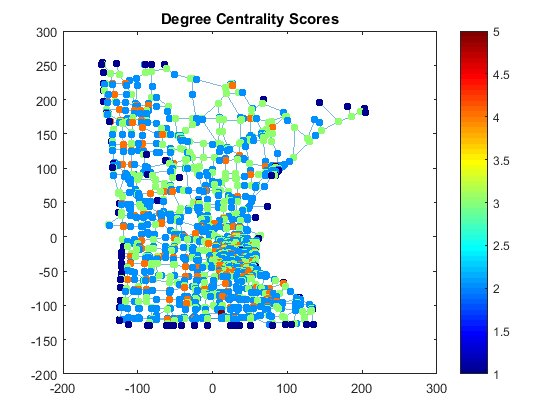
\includegraphics[scale=0.35]{figures/degreecentr.png}}
\end{tabular}
\vspace{-0.5cm}
\caption{Display of Minnesota Road Net -- no centrality displayed (left), degree centrality $C_{D}$ (right)}
\vspace{-0.2cm}
    \href{https://github.com/QuantLet/METISNET/tree/master/METISNET-centralitycomparison}{\quantnet METISNET-centralitycomparison}
\end{figure}
}

\frame{
\frametitle{Minnesota Road Networks}
\begin{figure}
\begin{tabular}{cc}
\subfloat{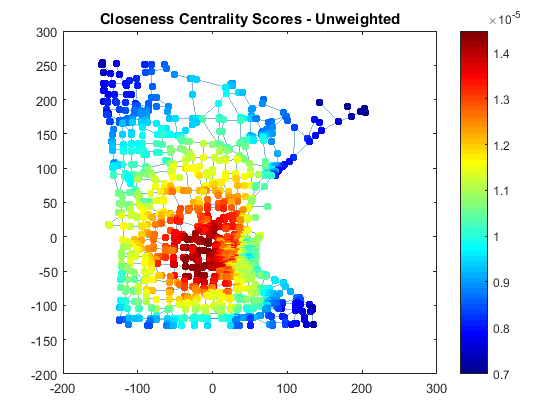
\includegraphics[scale=0.35]{figures/closeness_unweighted.png}}
&\subfloat{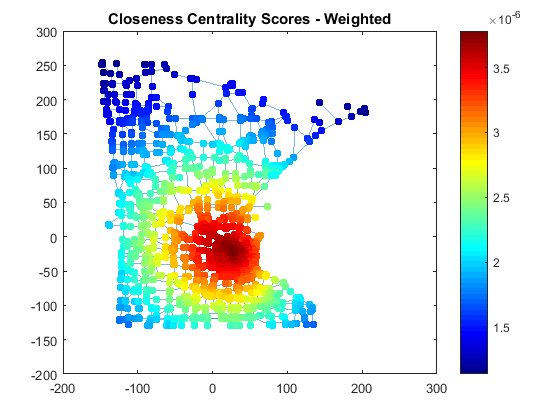
\includegraphics[scale=0.35]{figures/closeness_weighted.png}}
\end{tabular}
\vspace{-0.5cm}
\caption{Display of Minnesota Road Net -- closeness centrality unweighted (left), closeness centrality weighted (right)}
\vspace{-0.2cm}
    \href{https://github.com/QuantLet/METISNET/tree/master/METISNET-centralitycomparison}{\quantnet METISNET-centralitycomparison}
\end{figure}
}

\frame{
\frametitle{Minnesota Road Networks}
\begin{figure}
\begin{tabular}{cc}
\subfloat{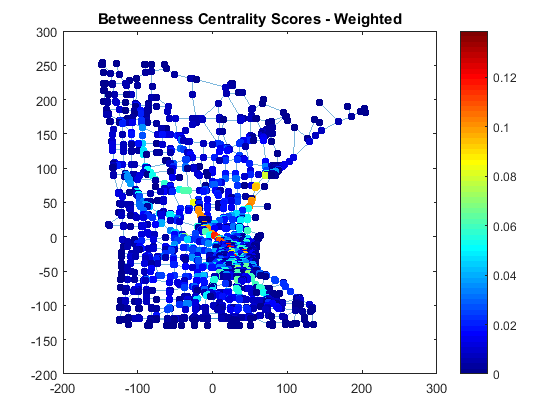
\includegraphics[scale=0.35]{figures/btwness_unweighted.png}}
&\subfloat{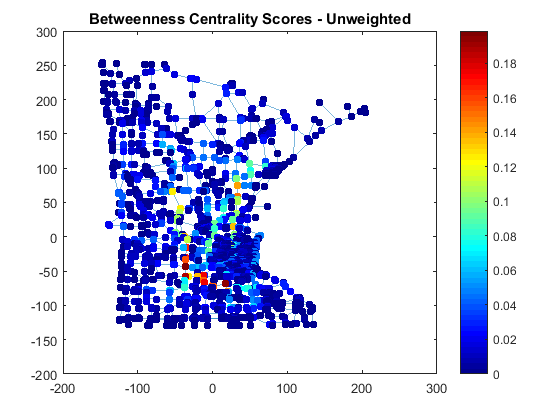
\includegraphics[scale=0.35]{figures/btwness_weighted.png}}
\end{tabular}
\vspace{-0.5cm}
\caption{Display of Minnesota Road Net -- betweenness centrality unweighted (left), betweenness centrality weighted (right)}
\vspace{-0.2cm}
    \href{https://github.com/QuantLet/METISNET/tree/master/METISNET-centralitycomparison}{\quantnet METISNET-centralitycomparison}
\end{figure}
}

\frame{
\frametitle{Minnesota Road Networks}
\begin{figure}
\begin{tabular}{cc}
\subfloat{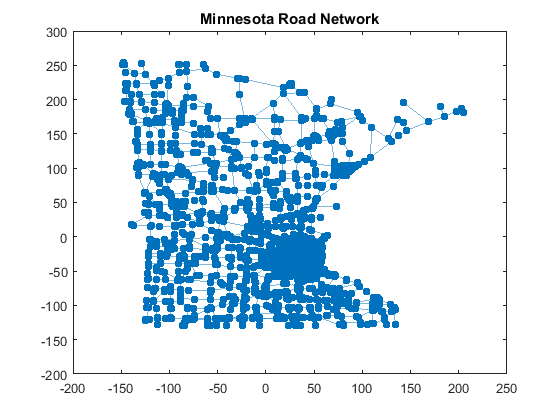
\includegraphics[scale=0.35]{figures/minnesotaroadnet.png}}
&\subfloat{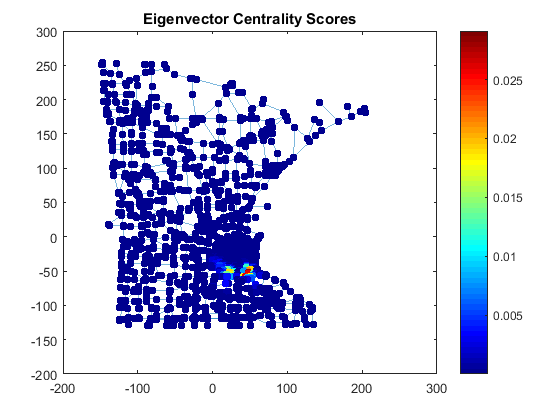
\includegraphics[scale=0.35]{figures/eigenctr.png}}
\end{tabular}
\vspace{-0.2cm}
\caption{Display of Minnesota Road Net -- no centrality displayed (left), eigenvector centrality $C_{E}$(right)}
\vspace{-0.5cm}
    \href{https://github.com/QuantLet/METISNET/tree/master/METISNET-centralitycomparison}{\quantnet MEITSNET-centralitycomparison}
\end{figure}
}

\frame[plain]{
\titlepage
}


%}

\end{document}